\documentclass[10pt,openany]{amsbook}

%%%%%%%%%%%%%%%%%%%%%%%%%%%%%%%%%%%%%%%%%%%%%%%%%%%%%%%%%%%%%%%%%%%%%% 
\usepackage{amsmath,amssymb,amsfonts}
\usepackage{epsfig}  		% For postscript
%\usepackage{showkeys}
\usepackage{booktabs}
\usepackage{hyperref}
\usepackage[font=small,labelfont=bf]{caption}
\usepackage[subrefformat=parens]{subcaption}
%\usepackage[titletoc]{appendix}
\usepackage{minitoc}
\usepackage{bm}

\usepackage{graphicx}
\usepackage{tabularx}

\usepackage[ruled, onelanguage]{algorithm2e}
\usepackage{multicol}

\usepackage{tikz}
\usepackage{etoolbox} % for \ifnumcomp
\usepackage{listofitems} % for \readlist to create arrays

\tikzset{>=latex} % for LaTeX arrow head
\colorlet{myred}{red!80!black}
\colorlet{myblue}{blue!80!black}
\colorlet{mygreen}{green!60!black}
\colorlet{mydarkred}{myred!40!black}
\colorlet{mydarkblue}{myblue!40!black}
\colorlet{mydarkgreen}{mygreen!40!black}
\tikzstyle{node}=[very thick,circle,draw=myblue,minimum size=22,inner sep=0.5,outer sep=0.6]
\tikzstyle{connect}=[->,thick,mydarkblue,shorten >=1]
\tikzset{ % node styles, numbered for easy mapping with \nstyle
  node 1/.style={node,mydarkgreen,draw=mygreen,fill=mygreen!25},
  node 2/.style={node,mydarkblue,draw=myblue,fill=myblue!20},
  node 3/.style={node,mydarkred,draw=myred,fill=myred!20},
}
\def\nstyle{int(\lay<\Nnodlen?min(2,\lay):3)}

\newcommand{\bbm}[1]{{\mathbf{#1}}}
\DeclareMathOperator*{\argmin}{argmin}   % Jan Hlavacek

\hypersetup{
    colorlinks,
    citecolor=blue,
    filecolor=black,
    linkcolor=blue,
    urlcolor=blue
}

\usepackage[a4paper,
            bindingoffset=0.2in,
            left=1in,
            right=1in,
            top=1in,
            bottom=1in,
            footskip=.25in]{geometry}

%%%%%%%%%%%%%%%%%%%%%%%%%%%%%%%%%%%%%%%%%%%%%%%%%%%%%%%%%%%%%%%%%%%%%%
\usepackage{lettrine}
\renewcommand{\LettrineTextFont}{\MakeUppercase}
\renewcommand{\thechapter}{\Roman{chapter}}

\makeatletter
\renewcommand\tocchapter[3]{%
  \indentlabel{\@ifnotempty{#2}{\ignorespaces#2.\quad}}#3\dotfill%
}
\renewcommand{\tocsection}[3]{%
  \indentlabel{\@ifnotempty{#2}{\ignorespaces#1 #2.\quad}}#3\dotfill%
}
\makeatother
%%%%%%%%%%%%%%%%%%%%%%%%%%%%%%%%%%%%%%%%%%%%%%%%%%%%%%%%%%%%%%%%%%%%%%

%%%%%%%%%%%%%%%%%%%%%%%%%%%%%%%%%%%%%%%%%%%%%%%%%%%%%%%%%%%%%%%%%%%%%%
\newlength{\bibitemsep}\setlength{\bibitemsep}{.5\baselineskip plus .05\baselineskip minus .05\baselineskip}
\newlength{\bibparskip}\setlength{\bibparskip}{0pt}
\let\oldthebibliography\thebibliography
\renewcommand\thebibliography[1]{%
  \oldthebibliography{#1}%
  \setlength{\parskip}{\bibitemsep}%
  \setlength{\itemsep}{\bibparskip}%
}
%%%%%%%%%%%%%%%%%%%%%%%%%%%%%%%%%%%%%%%%%%%%%%%%%%%%%%%%%%%%%%%%%%%%%%



\begin{document}

\begin{titlepage} % Suppresses displaying the page number on the title page and the subsequent page counts as page 1
	\newcommand{\HRule}{\rule{\linewidth}{0.5mm}} % Defines a new command for horizontal lines, change thickness here
	
	\center % Centre everything on the page
	
	%------------------------------------------------
	%	Headings
	%------------------------------------------------
	
	\textsc{\LARGE Université de Strasbourg}\\[2.5cm] % Main heading such as the name of your university/college
	
	%\textsc{\Large Master thesis}\\[0.5cm] % Major heading such as course name
	
	\textsc{\large Master Calcul Scientifique et Mathématiques de l'Information }\\[0.5cm] % Minor heading such as course title
	
	%------------------------------------------------
	%	Title
	%------------------------------------------------
	
	\HRule\\[0.4cm]
	
	{\huge\bfseries Reduced Order Modeling For Highly Nonlinear Partial Differential Equations 
    Using Physics Informed Neural Networks}\\[0.4cm] % Title of your document
	
	\HRule\\[1.5cm]
	
	%------------------------------------------------
	%	Author(s)
	%------------------------------------------------
	
	\begin{minipage}{0.4\textwidth}
		\begin{flushleft}
			\large
			\textit{Author}\\
			Vincent \textsc{Italiano} % Your name
		\end{flushleft}
	\end{minipage}
	~
	\begin{minipage}{0.4\textwidth}
		\begin{flushright}
			\large
			\textit{Supervisors}\\
			Emmanuel \textsc{Franck}\\ % Supervisor's name
            Victor \textsc{Michel-Dansac}\\ % Supervisor's name
            Hubert \textsc{Baty}\\ % Supervisor's name
            Vincent \textsc{Vigon} % Supervisor's name
		\end{flushright}
	\end{minipage}
	
	% If you don't want a supervisor, uncomment the two lines below and comment the code above
	%{\large\textit{Author}}\\
	%John \textsc{Smith} % Your name
	
	%------------------------------------------------
	%	Date
	%------------------------------------------------
	
	\vfill\vfill\vfill % Position the date 3/4 down the remaining page
	
	{\large From 14/02/2022 to 19/08/2022} % Date, change the \today to a set date if you want to be precise
	
	%------------------------------------------------
	%	Logo
	%------------------------------------------------
	
	%\vfill\vfill
	%
\includegraphics[width=0.2\textwidth]{img/logo_inria.jpg}\\[1cm] % Include a department/university logo - this will require the graphicx package
	 
	%----------------------------------------------------------------------------------------
	
	\vfill % Push the date up 1/4 of the remaining page
	
\end{titlepage}

\title[PINN's]{Physics informed Neural networks}
\author[V.Italiano]{Vincent Italiano}
%\xdef\shorttitle{\shorttitle{} -- report \noexpand\MakeUppercase{\shortauthors}}

%\maketitle
\frontmatter
\addtocontents{toc}{\protect\contentsline{chapter}{}{\textsc{\small Page}}{}}
\tableofcontents

\mainmatter
\addtocontents{toc}{\protect\contentsline{chapter}{Chapter}{}{}}
%%%%%%%%%%%%%%%%%%%%%%%%%%%%%%%%%%%%%%%%%%%%%%%%%%%%%%%%%%%%%%%%%%%%%%
\chapter{Introduction}
%%%%%%%%%%%%%%%%%%%%%%%%%%%%%%%%%%%%%%%%%%%%%%%%%%%%%%%%%%%%%%%%%%%%%%

\section{Context}

Inria is the French national research institute for digital science and technology. 
Established in 1967 at Rocquencourt, on a site that had previously been occupied by NATO, 
as the Institute for Research in IT and Automation (Iria), Inria’s mission is to accelerate, through digital research and innovation, 
the construction of France’s scientific, technological and industrial leadership in European dynamics 
(according to Inria’s website). It is composed by 10 research centers throughout France and even one center in Chile. 
Its headquarter is located in Rocquencourt, near Versailles. 
Today, more than 3,900 researchers and engineers work at Inria which hosts over 200 projects teams, 
most of which are shared with major research universities.

\begin{center}
    
\includegraphics[scale=0.2]{img/logo_inria.jpg}
\end{center}

My internship took place in one of those research teams, TONUS (TOkamaks and NUmerical Simulations), 
of the Nancy-Grand Est research center. 
The objective of this team is to deal with the mathematical and computing issues derived 
from kinetic and gyrokinetic modeling and simulations of collisionless plasmas. 
Together with the University of Strasbourg’s Institute for Advanced Mathematical Research (IRMA), 
they work on fluid plasma models; collisions; reduced, multi-scale and asymptotic models; electromagnetism. 
And more recently, the research team has been exploring AI solutions for the problems arising from the latter subjects.\\

My internship was done under the supervision of Emmanuel Franck (Inria), Victor Michel-Dansac (Inria), 
Hubert Baty (Strasbourg’s astronomical observatory), and Vincent Vigon (University of Strasbourg). We worked 
on the usage of deep learning methods to solve partial differential equations and the construction of reduced order method.

\section{Motivation}

Over the last decades, artificial neural networks have been used to solve problems in varied applied domains including 
image classification, 
handwriting recognition, speech recognition and translation, computer vision and many more \cite{Lecun}.
Despite the remarkable success in these areas, deep learning has not yet been widely used in the field of
scientific computing. However, more recently, solving partial differential equations via deep learning 
has emerged with a new class of artificial neural networks known as Physics-Informed Neural Networks \cite{raissi2017physicsI}.\\

To obtain the approximate solution of a partial differential equation via deep learning, a key step is to
constrain the neural network to minimize the partial differential equation residual, and several approaches
have been proposed to accomplish this. Compared to traditional mesh-based methods,
such as the finite volume method or the finite element method,
deep learning could be a mesh-free approach by taking advantage of automatic differentiation, 
and could break the curse of dimensionality. Another attractive feature of Physics-Informed Neural Networks
is that it can be used to solve inverse problems with minimum change and have been further 
extended to solve integro-differential equations, stochastic differential equations \cite{luetal} 
and more recently reduced-order modeling of nonlinear problems \cite{CHEN2021110666}.\\

\section{Research project}

The research project of the internship concerns the application of deep learning methods to solve magnetohydrodynamic equations.
These equations combine the Navier-Stokes equations for fluid dynamics with Maxwell’s equations for electromagnetism 
to form a mathematical theory for plasmas.  Magnetohydrodynamic helps us understand space plasmas in Earth
and planetary magnetospheres, as well as the physics of the Sun, solar wind, and stellar atmospheres. 
In fusion research, magnetohydrodynamic is crucial to the understanding of plasma equilibria and their
stability.\\

In particular, these partial differential equations are used by physicists to study the magnetic reconnection processes and 
are parameterized by the plasma resistivity $\eta$. 
The understanding of magnetic reconnection is a major goal of theoretical plasma physics in order to explain explosive events 
like solar/stellar flares, coronal mass ejections, and gamma-ray
flares in pulsar winds. \cite{Baty_2019}\\

However, the study of the reconnection process requires repeated model evaluations 
over a potentially large range of parameter values, and high-fidelity simulations remain  expensive.
Therefore, the goal of the internship is to developp an efficient reduced-order modeling for the magnetohydrodynamic equations
using the PINNs framework.\\

First of all, we applied the physics-informed neural networks to the 1-dimensional Burgers' equation and non-linear 
2-dimensional partial differential equation. 
We learned how to solve partial differential equations using this framework  and tested how all the parameters
affect the resolution. We also tried different methods to improve the training, using importance sampling.
Then we built a reduced model for the 1-dimensional Burgers equation with the viscosity as parameter.
Finally, we focused on magnetohydrodynamics and we chose to solve a problem called the tilt instability. 
We managed to solve this problem with physics-informed neural networks but we needed to include a lot of
simulation data in the training process and the research for good hyperparameters for the training was very long
and tedious. Due to lack of time, we were not able to design a reduced model which works for the initial problem. 

%%%%%%%%%%%%%%%%%%%%%%%%%%%%%%%%%%%%%%%%%%%%%%%%%%%%%%%%%%%%%%%%%%%%%%
\chapter{Physics informed neural networks}
%%%%%%%%%%%%%%%%%%%%%%%%%%%%%%%%%%%%%%%%%%%%%%%%%%%%%%%%%%%%%%%%%%%%%%

In this section, we introduce Physics informed neural networks (PINNS) \cite{raissi2017physicsI} and we detail the building blocks :
neural networks architecture, training, 
loss, etc.. We then make a comparison between PINNs and FEM and we show how to use PINNs to solve the 1D Burger's equations 
and a 2-dimensional non-linear PDE.

\section{What PINNs are}

Physics-Informed Neural Networks (PINNs) are neural networks used to solve problems involving Partial Differential Equations.
PINNs approximate PDE solutions by training a neural network to minimize a loss function; this loss contains terms 
reflecting the initial and boundary conditions and the PDE residual at selected points in the domain (called collocation point).\\

The PINN algorithm is essentially a mesh-free technique that finds PDE solutions by converting the problem of directly solving the governing equations into
a loss function optimization problem. It works by integrating the mathematical 
model into the network and reinforcing the loss function with a residual
term from the governing equation, which acts as a penalizing term to restrict
the space of acceptable solutions \cite{https://doi.org/10.48550/arxiv.2201.05624}.

\subsection{Problem setup}

We consider the following generic PDEs defined on a bounded continuous spatial domain $\Omega\in\mathbb{R}^d$ with boundary $\partial \Omega$:
\begin{align*}
\mathcal{N}[t,\bbm x, u] &= 0 \quad \text{ on } [0,T]\times\Omega\\
\mathcal{I}[\bbm x, u] &= 0 \quad \text{ on } \Omega\\
\mathcal{B}[t,\bbm x, u] &= 0 \quad \text{ on } [0,T]\times \partial\Omega
\tag{1}
\label{pde:1}
\end{align*} 

where $u$ represents the unknown solution, $\bm x \in \Omega$ is the spatial coordinate, $t$ is the time, $T$ is the time horizon,
$\mathcal{N}$ is a general differential operator that may consist of time derivatives, spatial derivatives, 
and linear and nonlinear terms. Also, $\mathcal{I}$ and $\mathcal{B}$ denote, 
respectively, the initial and boundary conditions which can be, Dirichlet, Neumann, Robin, or periodic boundary conditions.\\

A PINN is a neural network $u_{\bm \theta}$, which approximates the solution of the PDE (\ref{pde:1}),
where $\bm \theta$ is the set of model parameters.

\subsection{Deep neural network architecture}

Since \cite{raissi2017physicsI} and their original vanilla PINN, the majority of PINNs have used feed-forward neural networks (FFNN).\\

A feed-forward neural network, is a collection of neurons organized in layers that perform calculations sequentially through the layers.
Neurons in adjacent layers are connected, whereas neurons inside a single layer are not linked (See Figure \ref{fig:FFNN}). Each
neuron is a mathematical operation that applies an activation function to the weighted sum of its own inputs plus a bias factor. \\

Let $\mathcal{N}^L(\bbm x) : \mathbb{R}^{d_{in}} \to \mathbb{R}^{d_{out}}$ be a $L$-layer neural network, with $N_l$ neurons in the $l$-th layer $(N_0 = d_{in}, N_L = d_{out})$. Let us
denote the weight matrix and bias vector in the l-th layer by $\bbm W^l \in \mathbb{R}^{N_l \times N_{l-1}}$ and
$\bbm b^l \in \mathbb{R}^{N_l}$ , respectively. Given a nonlinear activation function $\sigma$, which is applied
element-wisely, the FNN is recursively defined as follows :
\begin{align*}
\text {input layer :} & \quad \mathcal{N}^0(\bbm x) = \bbm x \in  \mathbb{R}^{d_{in}}\\
\text {hidden layers :} & \quad \mathcal{N}^l(\bbm x) = \sigma (\bbm W^l \mathcal{N}^{l-1}(\bbm x) + \bbm b^l)\in \mathbb{R}^{N_l} \quad \text{for } 1\leq l \leq L-1\\
\text {output layer :} & \quad \mathcal{N}^L(\bbm x) = \bbm W^L \mathcal{N}^{L-1}(\bbm x) + \bbm b^L \in \mathbb{R}^{d_{out}}
\end{align*}

In this case,  $\bm \theta = \{\bbm W^l, \bbm b^l\}_{1\leq l\leq L}$ is the set of all weight 
matrices and bias vectors in the neural network.

\begin{figure}[h!]
    \begin{center}
        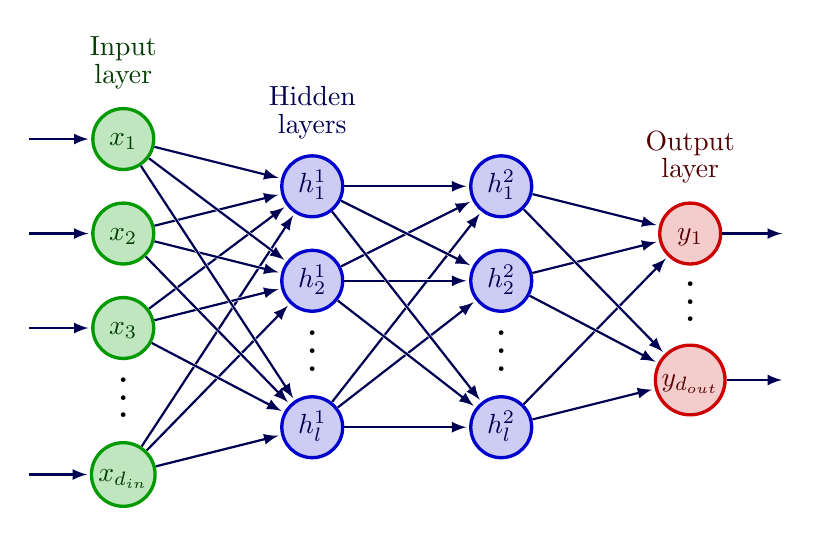
\begin{tikzpicture}[x=2.4cm,y=1.2cm]
            \readlist\Nnod{4,3,3,2} % array of number of nodes per layer
            \readlist\Nstr{d_{in},l,d_{out}} % array of string number of nodes per layer
            \readlist\Cstr{x,h^{\prev},y} % array of coefficient symbol per layer
            \def\yshift{0.55} % shift last node for dots
            
            % LOOP over LAYERS
            \foreachitem \N \in \Nnod{
              \def\lay{\Ncnt} % alias of index of current layer
              \pgfmathsetmacro\prev{int(\Ncnt-1)} % number of previous layer
              \foreach \i [evaluate={\c=int(\i==\N); \y=\N/2-\i-\c*\yshift;
                           \x=\lay; \n=\nstyle;
                           \index=(\i<\N?int(\i):"\Nstr[\n]");}] in {1,...,\N}{ % loop over nodes
                % NODES
                \node[node \n] (N\lay-\i) at (\x,\y) {$\strut\Cstr[\n]_{\index}$};
                
                % CONNECTIONS
                \ifnumcomp{\lay}{>}{1}{ % connect to previous layer
                  \foreach \j in {1,...,\Nnod[\prev]}{ % loop over nodes in previous layer
                    \draw[white,line width=1.2,shorten >=1] (N\prev-\j) -- (N\lay-\i);
                    \draw[connect] (N\prev-\j) -- (N\lay-\i);
                  }
                  \ifnum \lay=\Nnodlen
                    \draw[connect] (N\lay-\i) --++ (0.5,0); % arrows out
                  \fi
                }{
                  \draw[connect] (0.5,\y) -- (N\lay-\i); % arrows in
                }
                
              }
              \path (N\lay-\N) --++ (0,1+\yshift) node[midway,scale=1.6] {$\vdots$}; % dots
            }
            
            % LABELS
            \node[above=3,align=center,mydarkgreen] at (N1-1.90) {Input\\[-0.2em]layer};
            \node[above=2,align=center,mydarkblue] at (N2-1.90) {Hidden\\[-0.2em]layers};
            \node[above=3,align=center,mydarkred] at (N\Nnodlen-1.90) {Output\\[-0.2em]layer};
            
          \end{tikzpicture}
    \end{center}
    \caption{Feed forward neural network with 2 hidden layers.}
    \label{fig:FFNN}
\end{figure}

Note that some researchers have experimented with different types of neural networks like CNN and RNN, 
and some research papers used PINNs  with multiple fully connected networks blended together, 
e.g. to approximate specific equation of a larger mathematical model. 
(An architecture composed of five FFNNs is proposed by \cite{HAGHIGHAT2021113741}.
Instead of a single neural network across the entire domain, \cite{https://doi.org/10.48550/arxiv.2107.07871} 
suggests using multiple neural networks, one for each subdomain.)

\subsection{Training PINNs}
\label{sec:training}

Let us consider the following non-negative residuals, defined over the entire spatial and temporal domains

\begin{align*}
    r_{\mathcal{N}}(\bm \theta) &= \int_{[0,T]\times\Omega} \mathcal{N}[t,\bbm x, u_{\bm \theta}]^2 \mathrm{d}t\mathrm{d}\bbm x \\
    r_{\mathcal{I}}(\bm \theta) &= \int_{\Omega} \mathcal{I}[\bbm x, u_{\bm \theta}]^2 \mathrm{d}\bbm x \\
    r_{\mathcal{B}}(\bm \theta) &= \int_{[0,T]\times\partial\Omega} \mathcal{B}[t,\bbm x, u_{\bm \theta}]^2 \mathrm{d}t\mathrm{d}\bbm x\\
\end{align*}

Here, $r_{\mathcal{I}}(\bm \theta)$ and $r_{\mathcal{B}}(\bm \theta)$ quantifies the misfit of the neural network prediction 
and the initial/boundary conditions and $r_{\mathcal{N}}(\bm \theta)$ quantify how much the neural network is a solution to the PDE.\\

Therefore, the resolution of the PDE (\ref{pde:1}) is reduced to an optimization problem, where initial and boundary conditions can be 
viewed as constraints. 

\begin{equation}
    \bm \theta^* = \argmin_{\bm \theta} r_{\mathcal{N}}(\bm \theta) \quad s.t \quad r_{\mathcal{I}}(\bm \theta) = r_{\mathcal{B}}(\bm \theta) = 0
\end{equation}

This constrained optimization can be reformulated as an unconstrained optimization with a modified loss function
that also accommodates the constraints : 
\begin{equation}
    \bm \theta^* = \argmin_{\bm \theta} J(\bm \theta)
\end{equation}
where $J(\bm \theta)$ is defined by 
\begin{equation}
    J(\bm \theta) = r_{\mathcal{N}}(\bm \theta) + \lambda_1 r_{\mathcal{I}}(\bm \theta) + \lambda_2 r_{\mathcal{B}}(\bm \theta)
\end{equation}
in which $\lambda_1$ and $\lambda_2$ are weight parameters used to adjust the relative importance of each residual term.\\

To solve this unconstrained optimization problem, mini-batch Stochastic gradient descent (SGD) optimization algorithms
are used. In each iteration of a mini-batch SGD algorithm, the gradient of loss function $\nabla_{\bm \theta} J$ is
approximated through backpropagation using a batch of points of size $m$ in the input space, based
on which the neural network parameters are updated. 
More precisely,
we select according to a uniform distribution over the concerned domain \\

\begin{itemize}
    \item[1.] $N_r$ collocation points $\{t_j^r, \bbm x_j^r\}_{j=1}^{N_r}$ in $[0,T]\times\Omega$
    \item[2.] $N_0$ initial points $\{\bbm x_j^0\}_{j=1}^{N_0}$ in $\Omega$
    \item[3.] $N_b$ boundary points $\{t_j^b, \bbm x_j^b\}_{j=1}^{N_b}$ in $[0,T]\times\partial\Omega$
\end{itemize}
and at the $i$th iteration, we select a batch of $m$ collocation points and compute the loss function as a Monte-Carlo estimation 

\begin{align}
    J(\bm \theta) \simeq \frac{1}{m} \sum_{j=1}^{m} \mathcal{N}[t_j^r,\bbm x_j^r, u_{\bm \theta}(t_j^r,\bbm x_j^r)]^2
    + \frac{\lambda_1}{N_0} \sum_{j=1}^{N_0} \mathcal{I}[\bbm x_j^0, u_{\bm \theta}(0, \bbm x_j^0)]^2  
    + \frac{\lambda_2}{N_b} \sum_{j=1}^{N_b} \mathcal{B}[t_j^b,\bbm x_j^b, u_{\bm \theta}(t_j^b,\bbm x_j^b)]^2 
    \label{eq:LOSS}
\end{align}

At the $i$th iteration, the model parameters are updated according to
\begin{equation}
\bm \theta^{i+1} = \bm \theta^i - \eta^i \nabla_{\bm \theta}J(\bm \theta^i)
\label{eq:gradientstep}
\end{equation}

where $\eta^i$ is the step size in the $i$th iteration.\\

\begin{algorithm}[H]
    Sample $N_r$ collocation points from $[0,T]\times\Omega$, 
    $N_0$ points from $\Omega$ and $N_b$ points from $[0,T]\times\partial\Omega$\\
    Specify optimizer hyper-parameters, and error tolerance $\varepsilon$.\\
    \While{$J(\bm \theta^i)>\varepsilon$ }{
        Randomly select a batch of $m$ points out of the $N_r$ collocation points according to a uniform
        distribution.\\
        Compute the loss function using equation \ref{eq:LOSS}.\\
        Take a descent step (Equation \ref{eq:gradientstep}).\\
    }
    \caption{PINNs training}
    \label{algo:1}
\end{algorithm}

Moreover, to evaluate the loss function $J(\bm \theta)$ at the collocation points, we need to compute the derivatives of the network’s 
output with respect to its inputs. We use automatic differentiation  as it is the best choice among 
the four possible methods for computing the derivatives: 
(1) hand-coded analytical derivative; (2) symbolic
differentiation;
(3) finite difference or other numerical approximations; (4) automatic differentiation.\\

\begin{figure}[h!]
    \begin{center}
        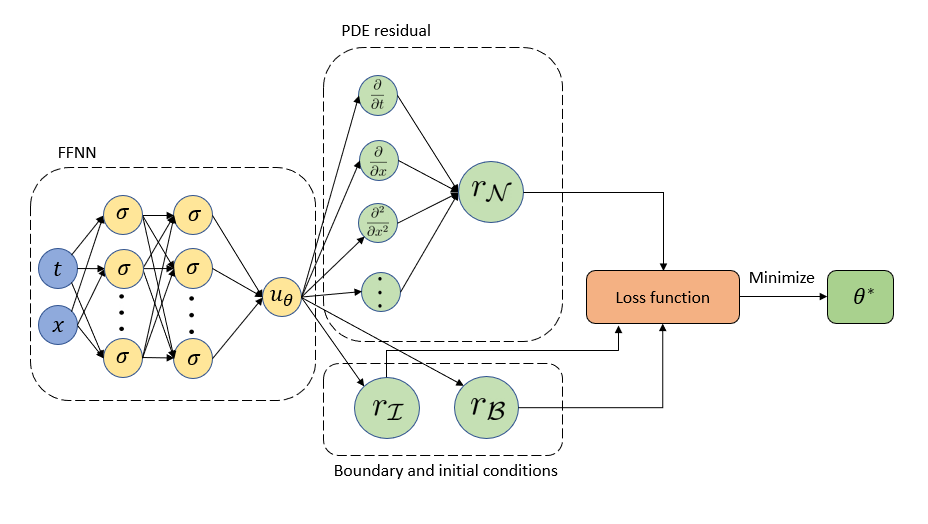
\includegraphics[scale=0.6]{img/schema.png}
    \caption{Schematic of a PINN for solving a PDE}
    \label{fig:PINNS}
    \end{center}
\end{figure}

\section{Comparison between PINNs and other numerical methods}

Here we compare the PINNs method to the other classical numerical methods \cite{luetal}, in particular to 
FEM and Finite Volume Method as they are the most frequently used.\\

\begin{itemize}
\item In classical numerical methods, the solution is approximated by a piecewise polynomial or constant function 
with point values to be determined, while in PINNs we construct a neural network parameterized by weights and biases.
\item Classical numerical methods requires a mesh generation, whereas PINN is totally mesh-free,
and we can use either a grid or random points.
\item PINNs' computational cost does not grow with the number of grid points. 
Furthermore, the trained PINN network may be used to predict values on simulated grids of various
resolutions without retraining. 
\item Classical numerical methods convert a PDE to an algebraic system (using the stiffness matrix and
mass matrix in FEM for example), while PINNs embed the PDE and boundary conditions into the
loss function.
\item In the last step, an algebraic system is solved exactly by a linear
solver, but the network in PINNs is learned by a gradient-based optimizer.
\item PINNs approximate the function and its derivatives
nonlinearly.
\end{itemize}

\section{Example}

In this section, we show how PINNs can solve PDEs with two examples: the 1-dimensional Burgers' equations, 
and a 2-dimensional PDE. The training is performed using TensorFlow on a NVIDIA Tesla V100-PCIE-16GB GPU.

\subsection{Burgers equation}

As a first example, let us consider the Burgers' equation. This equation arises
in various areas of applied mathematics, including fluid mechanics, gas dynamics, and traffic flow.\\

We consider the one dimensional Burger’s equation on the spatial domain $\Omega = [-1,1]$ and $t\in [0,1]$,
along with Dirichlet boundary conditions :

$$
\begin{cases}
    \partial_t u + \frac{1}{2}\partial_x u^2 = \nu \partial_{xx}u \quad \text{ on } [0,1]\times\Omega\\
    u(0,x) = \sin(\pi x) \quad \forall x \in \Omega\\
    u(t,-1) = u(t,1) = 0 \quad \forall t \in [0,1]
\end{cases}
$$
where $\nu$ is the viscosity. It is known that, for small values of
the viscosity parameter, Burgers’ equation can lead to shock formation that
is hard to solve using classical numerical methods.
We compare the solution of the Burgers' equation obtained using PINNs to a 
reference solution computed using finite volume method. \\

For a viscosity value of $\nu=10^{-3}$, we learn the solution by training all 3021 parameters of a 9-layer FFNN, 
with 20 neurons in each hidden layer and a hyperbolic tangent as activation function. 
We used $N_0 = N_b = 100$ randomly distributed initial and boundary data, and $N_r = 1,000$ collocation points inside
the domain and we choose to minimize the loss functions using the Adam optimizer from Tensorflow.
Figure \ref{fig:burgers1} shows the solution of the Burgers' equation obtained using PINNs compared to the
reference solution at different time instants $t = 0.25, 0.50, 0.75$.
Figure \ref{fig:burgers1loss} shows the loss decreasing during the training and the distribution of training points
inside the domain.\\

For smaller viscosities, we need to increase the number of layers and neurons per layer, and also the number of collocation points
and initial/boundary points to achieve a similar level of accuracy. 
Figure \ref{fig:burgers2} shows the solution of the Burgers' equation obtained using PINNs compared to the
reference solution at different time instants $t = 0.25, 0.50, 0.75$ for a viscosity $\nu = 10^{-4}$. We used 
a 16-layer FFNN, with 40 neurons in each hidden layer and a hyperbolic tangent as activation function.
Also we used $N_0 = N_b = 10,000$ randomly distributed initial and boundary data, and $N_r = 30,000$.\\

\begin{figure}[h!]
    \centering
    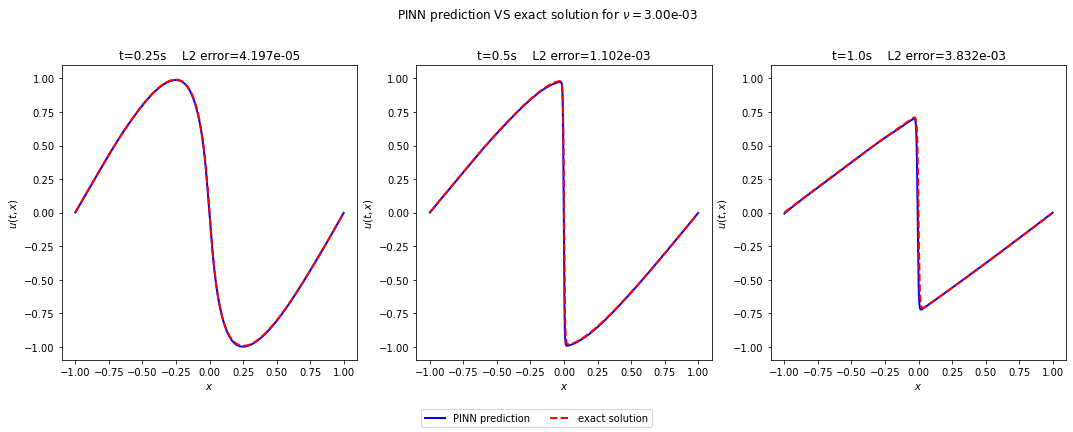
\includegraphics[scale=0.4]{img/burgers_nu1.png}
    \caption{Burgers' equation: Comparison of the predicted and exact
    solutions corresponding to three temporal snapshots. $\nu=10^{-3}$}
    \label{fig:burgers1}
\end{figure}

\begin{figure}[h!]
    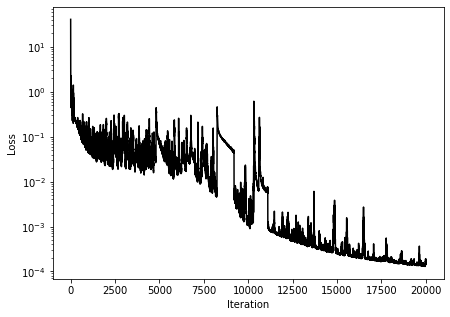
\includegraphics[width=0.49\textwidth,height=0.3\textwidth]{img/burgers_loss1.png}
    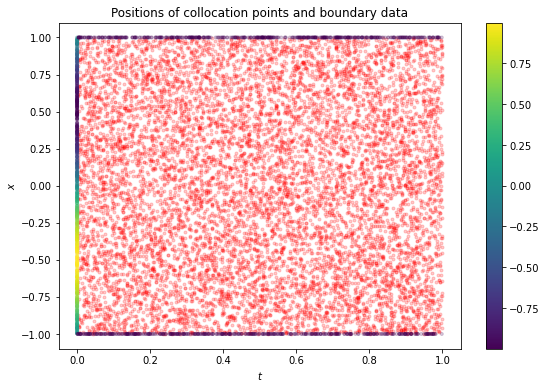
\includegraphics[width=0.49\textwidth,height=0.3\textwidth]{img/burgers_data.png}
    \caption{Loss history during training (left) distribution of training points. The colormap correspond to the values 
    of the initial condition function and the boundary condition (right)}
    \label{fig:burgers1loss}
\end{figure}

\begin{figure}[h!]
    \centering
    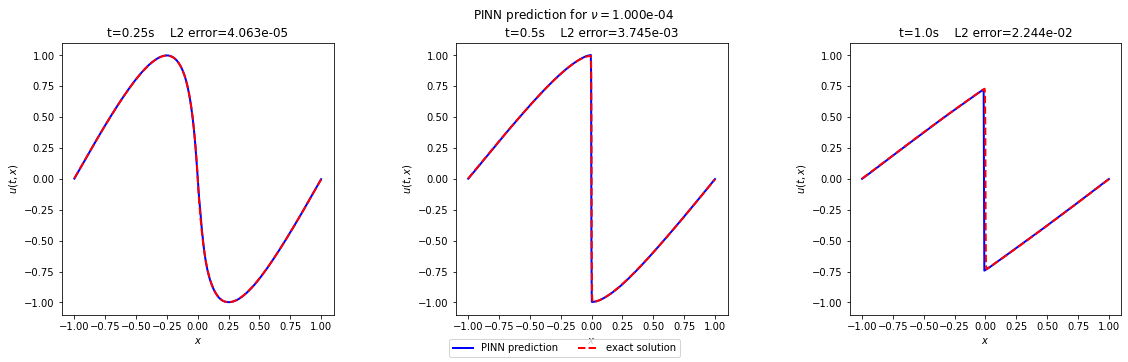
\includegraphics[scale=0.4]{img/burgers_nu2.png}
    \caption{Burgers' equation: Comparison of the predicted and exact
    solutions corresponding to three temporal snapshots. $\nu=10^{-4}$}
    \label{fig:burgers2}
\end{figure}

We must underline that, unlike any classical numerical method for solving 
PDEs, this prediction is obtained without any sort of discretization of the spatio-temporal domain. 
The exact solution for this problem is analytically available.

\subsection{2D case} 

Next,  we consider the following viscous 2-dimensional Burgers' equation on the spatial domain $\Omega = [0,1]\times[0,1]$
and $t\in [0,1.5]$.

\begin{equation}
        \begin{cases}
        \partial_t u + \frac{1}{2}\partial_x u^2  + \partial_y u = \nu \Delta u \quad \text{ sur } [0,1.5] \times \Omega\\
        u(0,x,y) = 1.5-2x \quad \forall (x,y) \in [0,1]\times[0,1]\\
        u(t,0,y) = 1.5, u(t,1,y) = -0.5, u(t,x,0) = 1.5-2x
    \end{cases}
    \label{eq:adv}
\end{equation}

where $\nu$ is the viscosity. Note that the quasi-linear term
involving shocks is one dimensional.\\

Figure \ref{fig:adv1} shows the solution of equation (\ref{eq:adv}) obtained using PINNs at different time instants 
$t = 0, 0.3, 0.6, 1.5$ for a viscosity $\nu = 10^{-3}$. We used a
8-layer FFNN, with 150 neurons in each hidden layer and a hyperbolic tangent as activation function.
Also, we used $N_0 = N_b = 10,000$ randomly distributed initial and boundary data, and $N_r = 30,000$.\\

\begin{figure}[h!]
    \begin{center}
        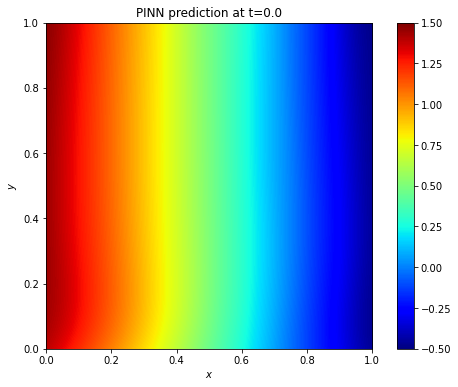
\includegraphics[width=.35\textwidth, height=0.5\textwidth, keepaspectratio]{img/adv_t0.png}
        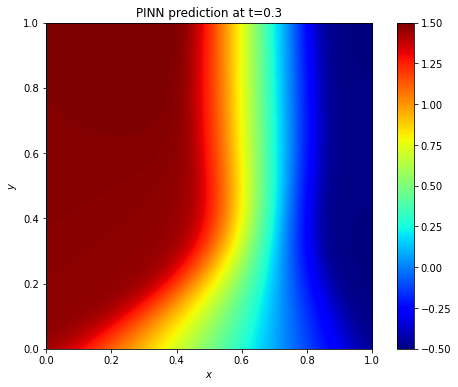
\includegraphics[width=.35\textwidth, height=0.5\textwidth, keepaspectratio]{img/adv_t3.png}
        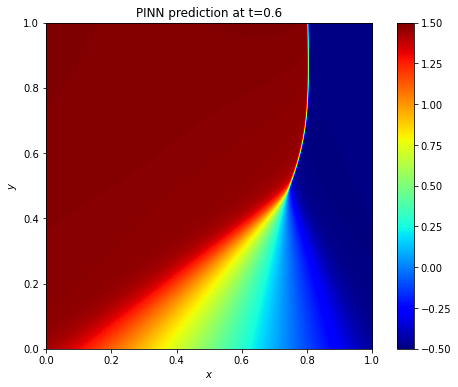
\includegraphics[width=.35\textwidth, height=0.5\textwidth, keepaspectratio]{img/adv_t6.png}
        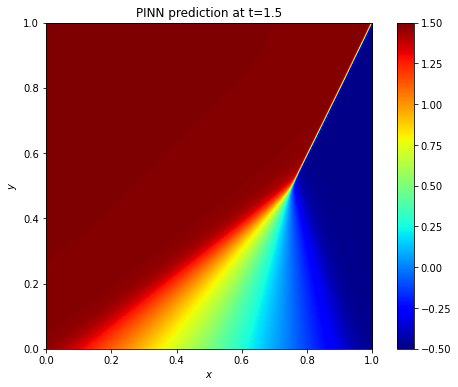
\includegraphics[width=.35\textwidth, height=0.5\textwidth, keepaspectratio]{img/adv_t15.png}
    \end{center}
    \caption{Predicted solutions of equation (\ref{eq:adv}) corresponding to four temporal snapshots. $\nu=10^{-3}$}
    \label{fig:adv1}
\end{figure}

We can see that a shock layer is formed, beginning at $(x = 0.75, y = 0.5)$ as a consequence of the steepening
of the slope solution when propagating upward and rightward, that has been initiated at the bottom layer. As time
advances, a final steady-state solution having an oblique shock layer between the previous point and the top-right
corner is obtained.\\

To check the validity of the PINNs solution, we have a reference solution, computed using finite element method.
Figure \ref{fig:adv2} compares the solution of equation (\ref{eq:adv}) obtained using PINNs and the reference solution for two time 
instants $t=0.8, 1.5$. It also shows the quadratic error between the two solutions. Figure \ref{fig:adv3} compares vertical slices of the solution obtained using PINNs and the reference solution at final time $t=1.5$, 
for four different values of $y$. 

\begin{figure}[h!]
    \begin{center}
        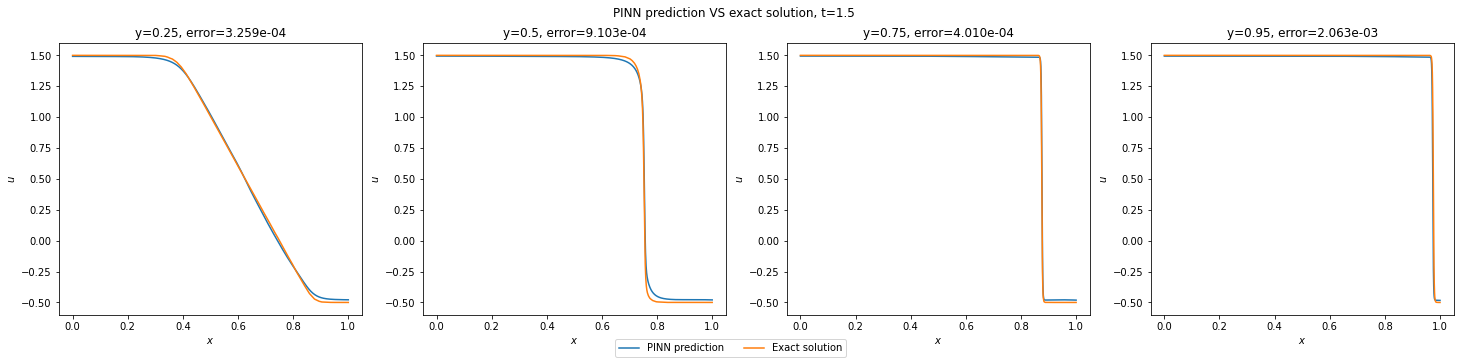
\includegraphics[width=1.\textwidth, height=0.4\textwidth, keepaspectratio]{img/adv_slice.png}
        \caption{Comparison of vertical slices of the predicted and exact solutions at final time $t=1.5$, 
        for four different values of $y$.}
        \label{fig:adv3}
    \end{center}
\end{figure}

\begin{figure}[h!]
    \begin{center}
        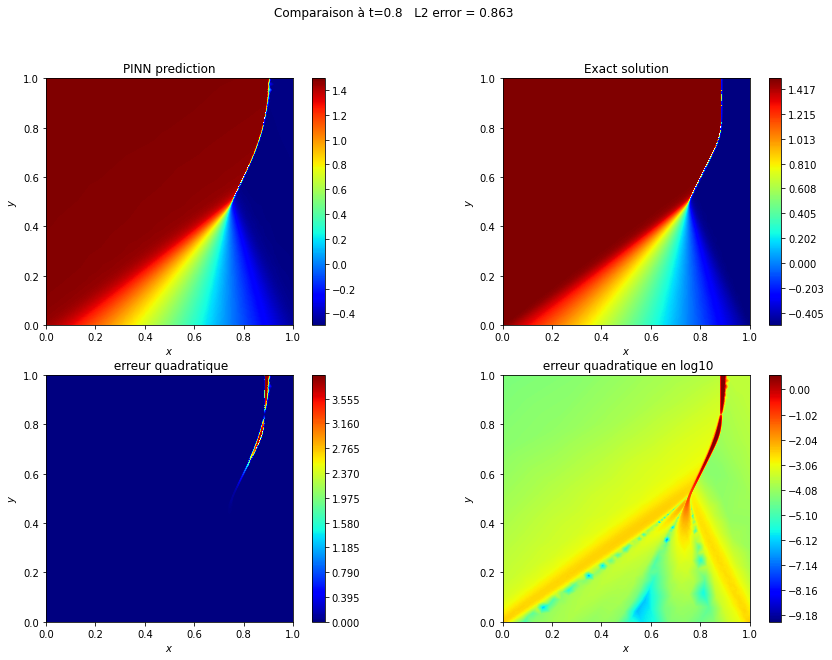
\includegraphics[width=.9\textwidth, keepaspectratio]{img/adv_error2.png}
        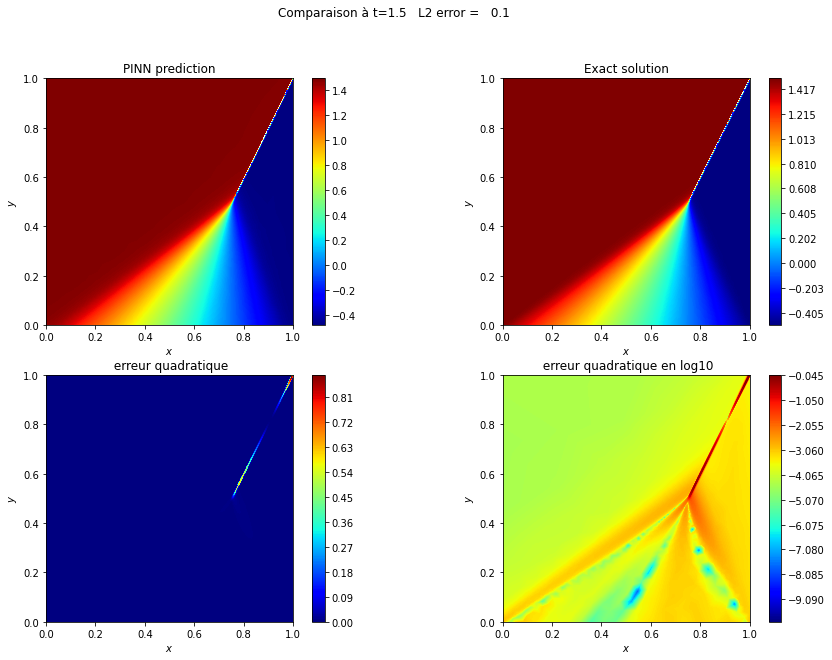
\includegraphics[width=.9\textwidth, keepaspectratio]{img/adv_error.png}
    \end{center}
    \caption{Comparison of the predicted and exact solutions corresponding to two temporal snapshots.}
    \label{fig:adv2}
\end{figure}

%%%%%%%%%%%%%%%%%%%%%%%%%%%%%%%%%%%%%%%%%%%%%%%%%%%%%%%%%%%%%%%%%%%%%%
\chapter{Reduced model for Burgers' equation}
%%%%%%%%%%%%%%%%%%%%%%%%%%%%%%%%%%%%%%%%%%%%%%%%%%%%%%%%%%%%%%%%%%%%%%

The first part of the intership was dedicated to the Burgers' equation. 
First we tried to improve PINNs training using importance sampling and looked for
good criteria to select collocation points during training. Then we built
a reduced model for the Burgers' equation where the viscosity is considered as a parameter.

%%%%%%%%%%%%%%%%%%%%%%%%%%%%%%%%%%%%%%%%%%%%%%%%%%%%%%%%%%%%%%%%%%%%%%
\section{Importance sampling}
%%%%%%%%%%%%%%%%%%%%%%%%%%%%%%%%%%%%%%%%%%%%%%%%%%%%%%%%%%%%%%%%%%%%%%

In this section, we present the work done to improve PINNs training using importance sampling, 
We propose to improve the distribution of residual points during the training process, 
conceptually similar to FEM refinement methods \cite{Nabian_2021} \cite{luetal}.

\subsection{Importance sampling}
As we discussed in section \ref{sec:training}, the training is performed using Monte-Carlo method 
to approximate the loss function $J(\bm \theta)$ and the collocation points are uniformly selected in the domain.
This works well for most cases, but it may not be efficient for some PDEs that exhibit
solutions with steep gradients \cite{failure}. For example, the Burgers' equation: intuitively
we should put more points near the sharp front to capture the discontinuity well.\\

In \cite{Nabian_2021}, they draw training samples from an alternative sampling distribution
based on the residual and we will follow their work.
They show that training of PINNs can be accelerated using an importance sampling approach where 
training samples are obtained from a distribution proportional to
the loss function. The idea is that we will add more residual points
in the locations where the PDE residual is large.
We also tried to sample training points from a distribution proportional to the entropy of the solution
and compare the two approaches. (see Figure \ref{fig:residuentropy})\\

\begin{figure}[h!]
    \begin{center}
        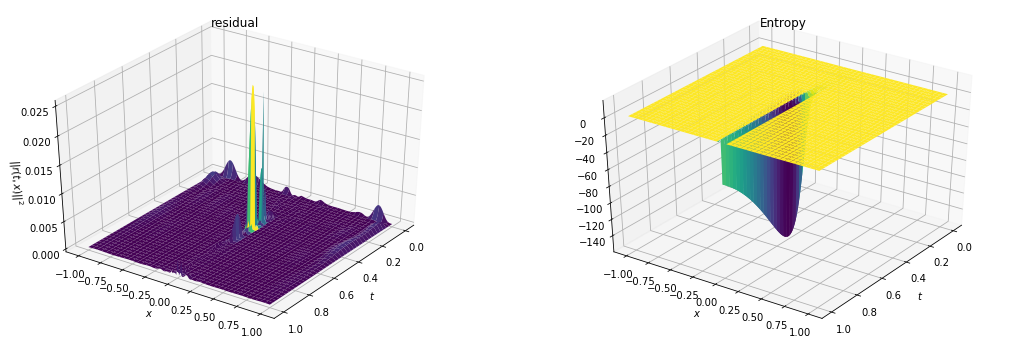
\includegraphics[width=1.\textwidth, height=0.3\textwidth]{img/adaptatif.png}
    \end{center}
    \caption{Surface plot of the PDE residual (left) 
    and the entropy (right)} associated to a PINN solution. The two distributions put more points 
    near the shock.
    \label{fig:residuentropy}
\end{figure}

This was effectively done by calculating the sampling distributions at the $i$th training step according to
\begin{equation}
    q_j^i = \frac{J(t_j^r, \bbm x_j^r; \bm \theta^i)}{\sum_{j=1}^N J(t_j^r, \bbm x_j^r; \bm \theta^i)} \quad \forall j=1, \ldots, N_r
\end{equation}
when using the residual, where 
$J(t_j^r, \bbm x_j^r; \bm \theta^i)  = \mathcal{N}[t_j^r,\bbm x_j^r, u_{\bm \theta^i}(t_j^r,\bbm x_j^r)]^2$. In the case 
of Burgers' equation, we have

\begin{equation}
    J(t_j^r, \bbm x_j^r; \bm \theta) = \Big[ \frac{\partial u_{\bm \theta}}{\partial t}(t_j^r,\bbm x_j^r) 
+ \frac{1}{2}\frac{\partial u_{\bm \theta}^2}{\partial x}(t_j^r,\bbm x_j^r)
- \nu \frac{\partial^2 u_{\bm \theta}}{\partial x^2}(t_j^r,\bbm x_j^r) \Big]^2
\end{equation}
And, 
\begin{equation}
    q_j^i = \frac{\mathcal{S}(t_j^r, \bbm x_j^r; \bm \theta^i)}{\sum_{j=1}^N \mathcal{S}(t_j^r, \bbm x_j^r; \bm \theta^i)} \quad \forall j=1, \ldots, N_r
\end{equation}

when using the entropy. Here $\mathcal{S}$ denotes the entropy function associated to the solution and, for the 
Burgers' equation, we have

\begin{equation}
    \mathcal{S}(t_j^r, \bbm x_j^r; \bm \theta) = \Big[ \frac{1}{2}\frac{\partial u_{\bm \theta}^2}{\partial t}(t_j^r,\bbm x_j^r) 
+ \frac{1}{3}\frac{\partial u_{\bm \theta}^3}{\partial x}(t_j^r,\bbm x_j^r)
- \nu \frac{\partial^2 u_{\bm \theta}^2}{\partial x^2}(t_j^r,\bbm x_j^r) \Big]^2
\end{equation}
Then we sample collocation points indices from a multinomial with probabilities 
$\bbm p^i = \{q_1^i, \ldots,q_{N_r}^i\}$ which represent the probability of each point in $\{t_j^r, \bbm x_j^r\}_{j=1}^{N_r}$
to be selected during the training step.\\

Although evaluation of the loss function for the entire set of collocation points in each iteration can
be very expensive, we use a piece-wise constant approximation to the loss
function to overcome this problem. That is, instead of evaluating the loss function at every collocation point, we evaluate the
loss only at a subset of points, hereinafter referred to as "seeds", denoted by $\{t_s, \bbm x_s\}_{s=1}^S$, with $S<N_r$. 
Next, using a nearest neighbor search algorithm (KD-Tree for example), for each collocation point, we identified the
nearest seed, and set the loss value at that collocation point equal to the loss at the nearest
seed. This is equivalent to generating a Voronoi tesselation using the seeds, 
and using a constant approximation for loss within each Voronoi cell.

Moreover, compared to \cite{Nabian_2021}, where they used very smooth PDEs, we want to apply the importance sampling method to the 
Burgers' equation. We still need to sample some collocation points uniformly 
otherwise almost all the points would be along the shock at each training step leading to a bad training.

Algorithm \ref{algo:IS} summarizes the steps for the proposed importance sampling method.\\

\begin{algorithm}[H]
    Sample $N_r$ collocation points from $[0,T]\times\Omega$, $S$ seeds from $[0,T]\times\Omega$,
    $N_0$ points from $\Omega$ and $N_b$ points from $[0,T]\times\partial\Omega$.\\
    For each collocation point, find the nearest seed.\\
    Specify optimizer hyper-parameters, batch size $m$, ratio of uniformly sampled points $\alpha$ and error tolerance $\varepsilon$.\\
    \While{$J(\bm \theta^{(i)})>\varepsilon$}{
        Compute the loss value at each seed.\\
        Compute the probability vector $\bbm p^{(i)} = \{q_1^i, \ldots,q_{N_r}^i\}$ according to the 
        selected criterion.\\
        Select $(1-\alpha) m$ collocation points out of the $N_r$ according to the multinomial law of parameter $\bbm p^{(i)}$.\\
        Select $\alpha m$ collocation points  out of the $N_r$ according to uniform distribution.\\
        Take a descent step.\\
    }
    \caption{Efficient training of PINNs using importance sampling}
    \label{algo:IS}
\end{algorithm}

\subsection{Results}
Here we compare the performance of the importance sampling method using residual and entropy with
the classical uniform method.\\

First of all, we note that the parameter $\alpha$ must be at least equal to $10\%$, otherwise 
almost all the points would be along the shock at each training step leading to a bad training. Higher values for $\alpha$ 
do not lead to much better results. From now on we will always choose $\alpha = 10\%$.\\

Next, we tested with a challenging viscosity $\nu = 10^{-4}$. Table \ref{table:resentr1} shows the minimal loss value 
obtained using the different algorithms, for different values of $N_r$. For each simulation
we train for 20,000 iterations a FFNN with 8 hidden layers and 64 neurons per layer.
We used the following hyperparameters: 
batch size is set to 3,000, learning rate is initially set to 
$10^{-4}$ and follows an exponential decay of factor $0.98$ every $200$ step.\\

\begin{table}[ht!]
    \centering
    \begin{tabular}{c c c c }
        \toprule
         & uniform sampling & IS using residual & IS using entropy\\
        \midrule
        10,000 points  & $9.44^{-2}$ & $4.31^{-2}$ & $7.87^{-2}$\\
        20,000 points  & $7.04^{-3}$ & $8.51^{-3}$ & $2.15^{-2}$\\
        40,000 points  & $6.53^{-3}$ & $3.05^{-3}$ & $1.47^{-3}$\\
        100,000 points & $4.75^{-3}$ & $7.48^{-4}$ & $5.32^{-4}$\\
        \bottomrule\\
    \end{tabular}
    \caption{Best loss reach during training. $\nu = 10^{-4}$}
    \label{table:resentr1}
\end{table}

We can see that importance sampling  is in general better than uniform sampling and 
importance sampling with entropy performs better than with residual when the number of collocation points is large. 
However, it is challenging, in general, to design a good distribution to sample collocation points
for problems whose solution is unknown (e.g when we do not know the entropy function), thus the residual method is prefered.

\section{Reduced model}

In this section we build a reduced order model coupled with PINNs to solve the Burgers' equation
with viscosity as a parameter. As a result, we reach an accuracy approaching $10^{-4}$ using a 
single PINN to predict the solution of the Burgers' equation for viscosities in the interval $[10^{-4}, 10^{-2}]$.\\

The advantage of PINNs over traditionnal numerical method is that 
the computational cost does not grow that much with the PDEs dimensions and the number of grid points. 
We exploit these properties to construct a reduced model using PINN : parametrized PDEs are viewed
as higher dimensional PDEs where the parameters are also variables.

\subsection{Results}

We adapt the previous PINNs setup to the new problem, adding $1$ input to the model, corresponding to 
the viscosity value. The new model is a $16$-layer FFNN, with $256$ neurons in each hidden layer and a hyperbolic tangent 
as activation function. Also we used $N_0 = N_b = 20,00$ randomly distributed initial and boundary data and $60,000$ collocation points.
The model is trained for viscosities in the interval $[10^{-4}, 10^{-2}]$ using the following hyperparameters : 
batch size is set to $3,000$, learning rate is initially set to 
$10^{-3}$ and follows an exponential decay of factor $0.97$ every $200$ step. 
We train for $20,000$ step. Figure \ref{fig:lossROMburgers} shows the loss decreasing during the training.\\

\begin{figure}[h!]
    \centering
    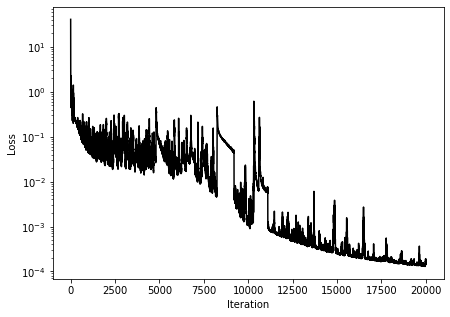
\includegraphics[scale=0.5]{img/lossROMburgers.png}
    \caption{Training loss of the PINN reduced model}
    \label{fig:lossROMburgers}
\end{figure}

Figure \ref{fig:ROMburgers} shows the predicted solution of the Burgers' equation for different viscosity values on the same plot, 
at different times $t=0, 0.25, 0.5, 1$. Figure \ref{fig:ROMburgers2} compares the model prediction to the solution computed using 
Finite Volume Method, for different time (horizontal) and different viscosities (vertical).

\begin{figure}[h!]
    \centering
    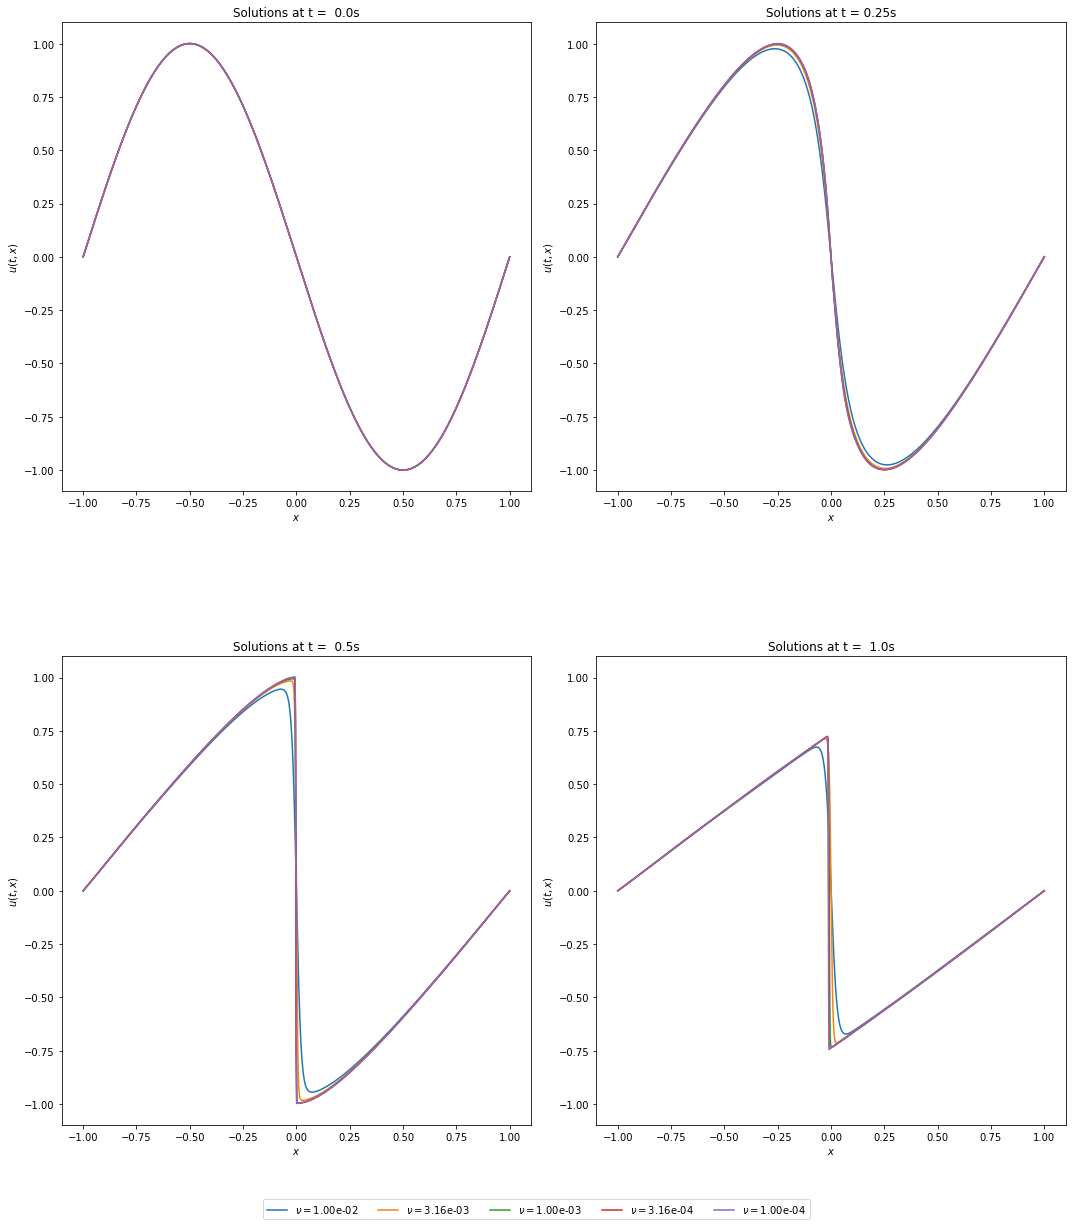
\includegraphics[scale=0.4]{img/t0.png}
    \caption{PINN prediction for different time and different viscosities}
    \label{fig:ROMburgers}
\end{figure}

\begin{figure}
    \begin{center}
        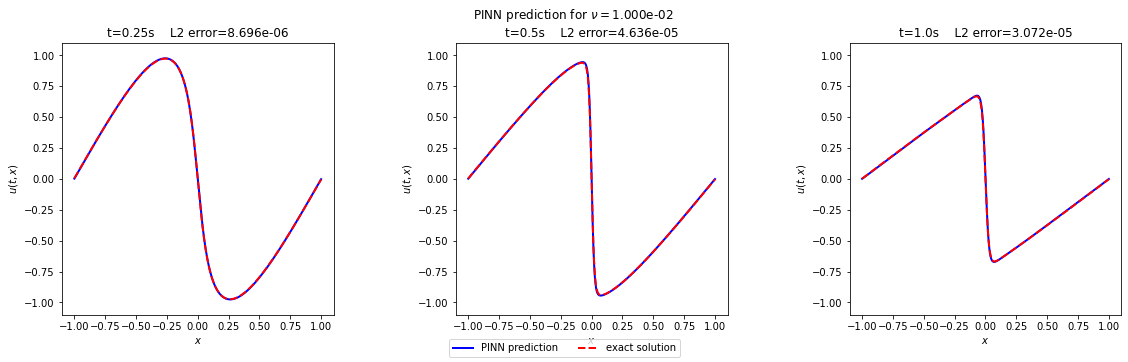
\includegraphics[width=.8\textwidth, height=0.4\textwidth, keepaspectratio]{img/burgers_multi1.png}
        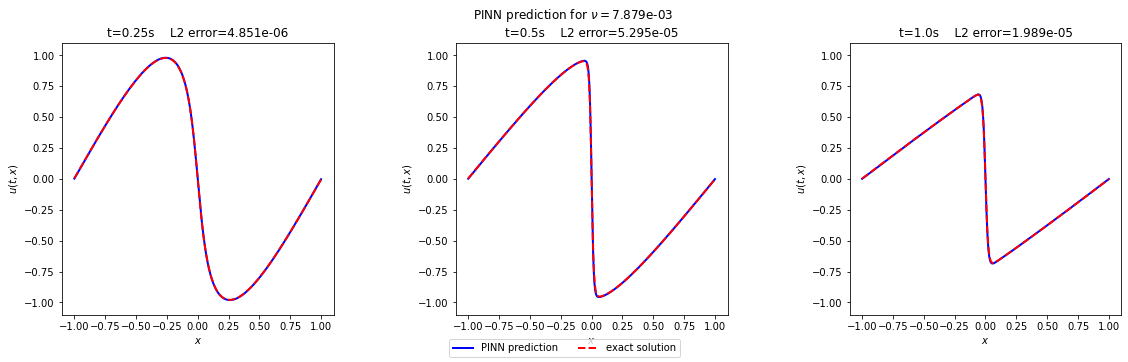
\includegraphics[width=.8\textwidth, height=0.4\textwidth, keepaspectratio]{img/burgers_multi2.png}
        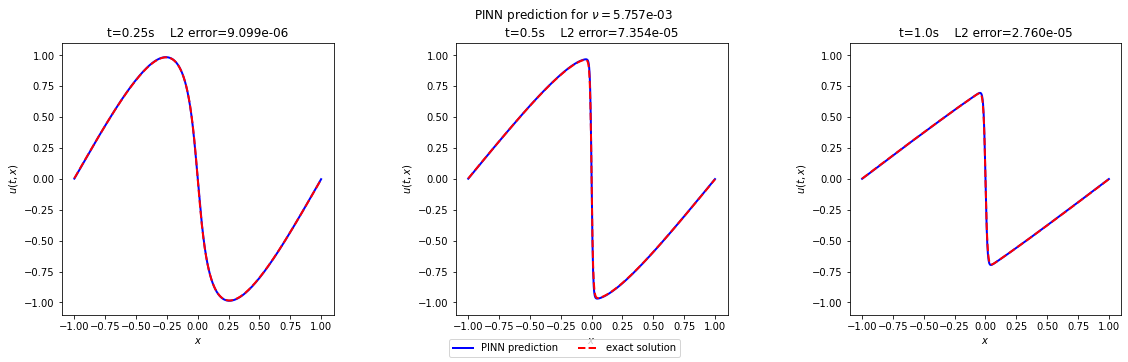
\includegraphics[width=.8\textwidth, height=0.4\textwidth, keepaspectratio]{img/burgers_multi3.png}
        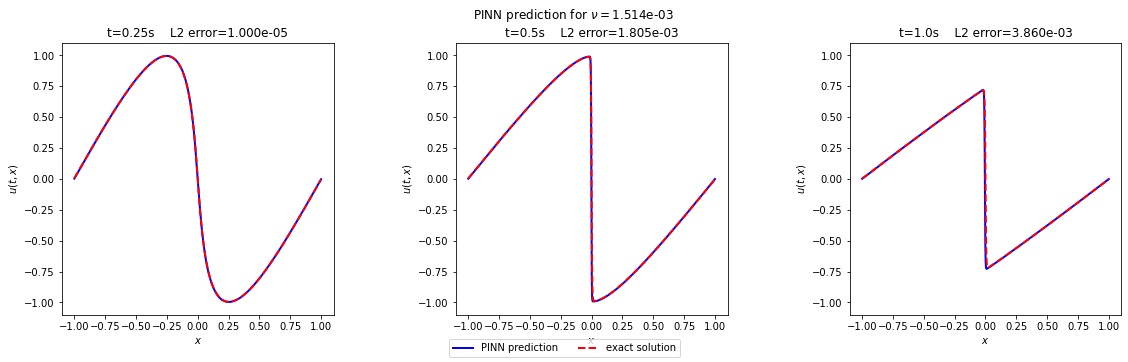
\includegraphics[width=.8\textwidth, height=0.4\textwidth, keepaspectratio]{img/burgers_multi4.png}
        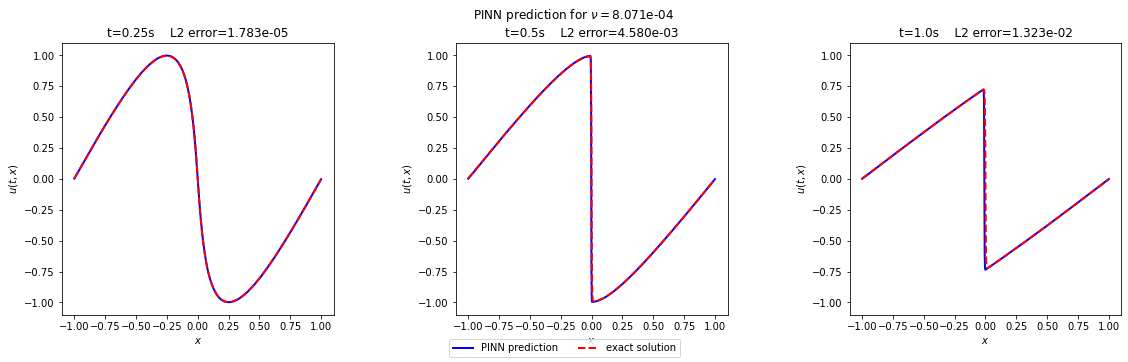
\includegraphics[width=.8\textwidth, height=0.4\textwidth, keepaspectratio]{img/burgers_multi5.png}
        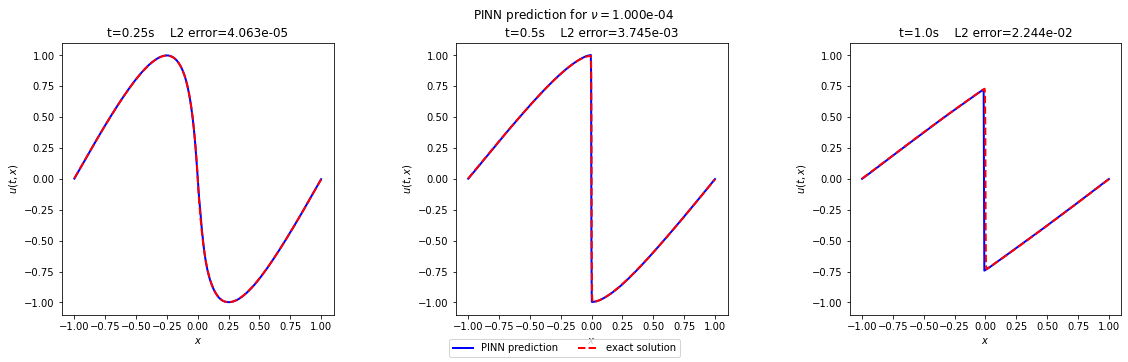
\includegraphics[width=.8\textwidth, height=0.4\textwidth, keepaspectratio]{img/burgers_multi6.png}
    \end{center}
    \caption{Solutions of Burgers' equation for different viscosity values, using a single neural network}
    \label{fig:ROMburgers2}
\end{figure}

%%%%%%%%%%%%%%%%%%%%%%%%%%%%%%%%%%%%%%%%%%%%%%%%%%%%%%%%%%%%%%%%%%%%%%
\chapter{Reduced order model for magnetohydrodynamics}

In the second part of the intership, we apply the PINNs framework to magnetohydrodynamics.
First, we introduce the magnetohydrodynamic and its governing equations, 
then we present the tilt instability configuration, and we present the results obtained 
using PINNs to solve this problem.

\section{What is magnetohydrodynamics}

Magnetohydrodynamics (MHD) is concerned with the flow of electrically 
conducting fluids in the presence of magnetic fields, either externally applied
or generated within the fluid by inductive action. The basic equations of MHD have been proposed by 
the Swedish physicist Hannes Alfven (1908-1995), who received the Nobel Prize in Physics in 1970 for 
\textit{"fundamental work and discoveries in 
magnetohydrodynamics with fruitful applications in different parts of plasma physics"}.

\begin{figure}[h!]
    \centering
    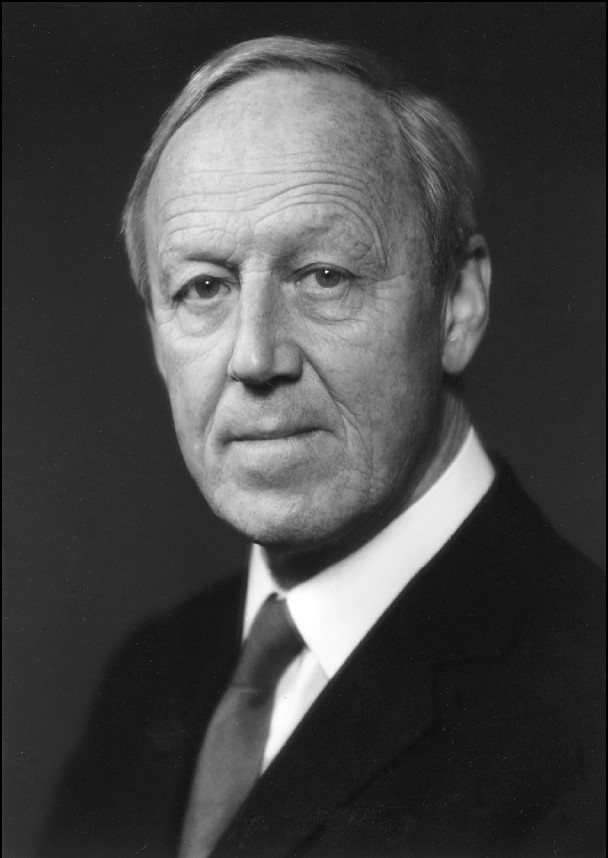
\includegraphics[scale=.15]{img/Alfven.jpg}
    \caption{Hannes Alfven (1908-1995)}
\end{figure}

MHD combines the Navier-Stokes equations for fluid dynamics
with Maxwell’s equations for electromagnetism to form a new mathematical theory for plasmas.
The main concept behind MHD  is that magnetic fields can induce currents in a moving conductive fluid,
which in turn creates forces on the fluid and influences the magnetic field itself.
MHD helps us understand space plasmas in Earth and planetary magnetospheres, as well as the physics of
the Sun, solar wind, and stellar atmospheres (Figure \ref{fig:flares}). In fusion research, MHD is crucial
to the understanding of plasma equilibria and their stability.

\begin{figure}[h!]
    \centering
    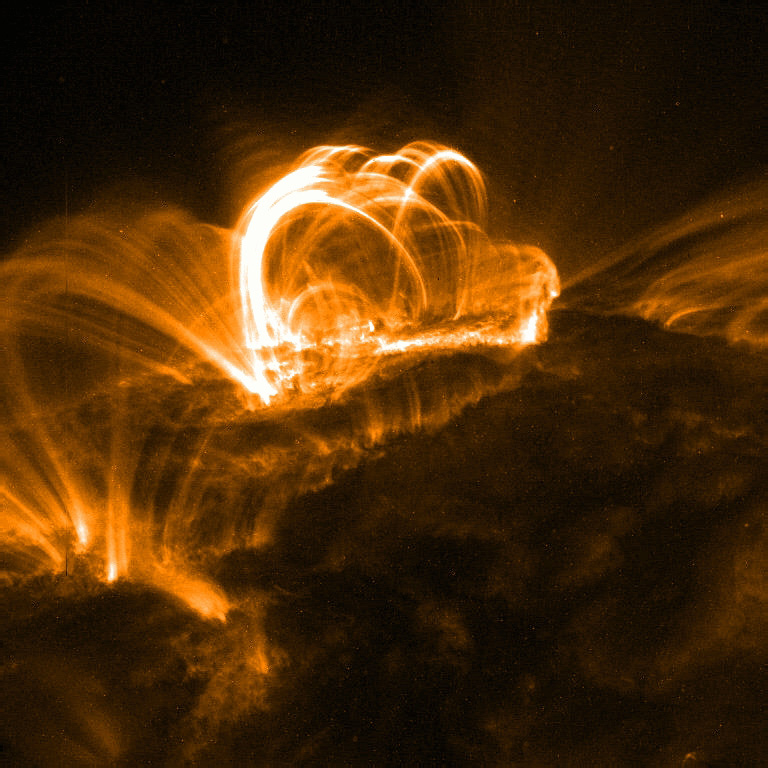
\includegraphics[scale=.2]{img/solar_flare.jpg}
    \caption{Solar flare, which can release particles and radiations. \\ Source : 
    \url{http://www-solar.mcs.st-and.ac.uk/~herbert/Before_2018/}}
    \label{fig:flares}
\end{figure}

\subsection{Equations of MHD}

The equations of magnetohydrodynamics are a reduction of the equations of fluid mechanics coupled with Maxwell’s equations.
Magnetohydrodynamics is composed of four equations, which consist of the basic conservation laws of mass, momentum and energy together 
with the induction equation for the magnetic field. \cite{baty:hal-03711796}\\

The first equation of MHD is the continuity
equation, which expresses the conservation of mass density 

\begin{equation}
    \frac{\partial \rho}{\partial t} + \nabla \cdot ( \rho \bbm V ) = 0
    \tag{a}
\end{equation}
where $\rho$ is the mass density and $\bbm V$ the flow velocity.\\

The second equation quantifies how the magnetic field acts on the hydrodynamic component.
\begin{equation}
    \rho \frac{\partial \bbm V}{\partial t} + \rho ( \bbm V \cdot \nabla)\bbm V =  \bbm J \times \bbm B - \nabla P + \mu \Delta \bbm V 
    \tag{b}
\end{equation}
Here $\bbm B$ is the magnetic field (subjected to the relation $\nabla \cdot \bbm B = 0$), 
$\bbm J = (\nabla \times \bbm B) / \mu_0$ the current density, $P$ is the fluid pressure,  $\bbm g$ the gravitational acceleration
and $\mu$ the dynamic viscosity coefficient of the fluid.\\

The other way around, the third equation quantifies how the flow velocity acts on the magnetic field.
\begin{equation}
    \frac{\partial \bbm B}{\partial t} = \nabla \times( \bbm V \times \bbm B) - \nabla \times (\bbm J/\sigma)
    \tag{c}
\end{equation}
where $\sigma$ is the electrical conductivity coefficient. This equation comes from the Maxwell-Faraday equation combining
with Ohm's law of conducting fluid.\\

The last equation is an equation of state, needed to close the set of relations. Neglecting the 
Joule heating, we can consider the following equation
\begin{equation}
    \frac{\partial P}{\partial t} + \bbm V \cdot \nabla P = - \Gamma P \nabla \cdot \bbm V
    \tag{c}
\end{equation}
where $\Gamma$ is the heat capacity ratio.\\

Finally, MHD is governed by the following set of equations,

\begin{align}
    & \frac{\partial \rho}{\partial t} + \nabla \cdot ( \rho \bbm V ) = 0 \\
    & \rho \frac{\partial \bbm V}{\partial t} + \rho ( \bbm V \cdot \nabla)\bbm V  =  \bbm J \times \bbm B - \nabla P + \mu \Delta \bbm V \\
    & \frac{\partial \bbm B}{\partial t}  = \nabla \times( \bbm V \times \bbm B) - \nabla \times (\bbm J/\sigma) \\
    & \frac{\partial P}{\partial t} + \bbm V \cdot \nabla P  = - \Gamma P \nabla \cdot \bbm V
\end{align}
with $\bbm J = (\nabla \times \bbm B) / \mu_0$  and $\nabla \cdot \bbm B = 0$.

\subsection{Reduced MHD}

Reduced magnetohydrodynamics is an incompressible fluid model of plasma behavior that is simpler than a full MHD model. 
It has the advantage of being computationally more efficient for many problems for which it is applicable.
It is a good approximation when the magnetic field is almost 
uniform and unidirectional : $ \bbm B \simeq B_z  \bbm e_z$. This situation may occur in many situations 
like loops in the solar atmosphere, Tokamaks, Magnetic clouds/flux ropes in the solar wind.\\

In this case, it can be shown that  the plasma is incompressible : $\nabla \cdot \bbm V = 0$ 
and its dynamics is constrained to a 2-dimensional plane:  i.e $\bbm V = V_x  \bbm e_x + V_y  \bbm e_y$. Thus 
the full MHD equations are reduced to simplified  equations in 2 dimensions,  reducing the numbers of scalar variables
from 8 to 4 but also leads to a better numerical handling.\\

\subsubsection{Flow-vorticy formulation}
We first consider reduced MHD equations written in flux-vorticity $(\psi - \omega)$ scalar variables,

\begin{align}
    & \frac{\partial \omega}{\partial t} + (\bbm V \cdot \nabla) \omega  = \frac{1}{\rho} (\bbm B \cdot \nabla)J  + \nu \Delta \omega \\
    & \frac{\partial \psi }{\partial t} + (\bbm V \cdot \nabla)  \psi = \eta \Delta  \psi  \\
    & \omega  = - \Delta \phi \\
    & \mu_0  J  =  - \Delta \psi 
\end{align}
Where we have introduced the two stream functions, $\phi(x, y)$ and $\psi(x, y)$, defined as 
$\bbm V = \nabla \phi \times \bbm e_z$ and $\bbm B = \nabla \psi \times \bbm e_z$
($\bbm e_z$ being the unit vector perpendicular to the $xOy$ simulation plane)
and $\omega$ and $J$ are the $z$ components of the vorticity and 
the current density vectors, as $\bm \omega = \nabla \times \bbm V$ and $\bbm J = (\nabla \times \bbm B) / \mu_0$. 
The coefficient $\eta = 1/(\mu_0 \sigma)$ is the magnetic resistivity.
Note that the thermal pressure gradient is naturally absent from our set of equations.\\

\subsubsection{Current-vorticity formulation}

Another formulation using current-vorticity $(J - \omega)$ exists, and is given by,

\begin{align}
    & \frac{\partial \omega}{\partial t} + (\bbm V \cdot \nabla) \omega  = \frac{1}{\rho} (\bbm B \cdot \nabla)J  + \nu \Delta \omega \\
    & \frac{\partial J }{\partial t} + (\bbm V \cdot \nabla) J = (\bbm B \cdot \nabla)\omega + \eta \Delta  J   + g(\phi,\psi)\\
    & \omega  = - \Delta \phi \\
    & \mu_0  J  =  - \Delta \psi 
\end{align}

with $g(\phi,\psi) = 2[\frac{\partial \psi}{\partial x}, \frac{\partial \phi}{\partial x}] + 
2[\frac{\partial \psi}{\partial y},\frac{\partial \phi}{\partial y}]$. This second formulation has advantages
over the first one, as the two evolution equations are more symmetric, thus facilitating the numerical matrices calculus
for linear solvers and there is no numerical instabilities due to the evaluation of the third order spatial derivative term
$(\bbm B \cdot \nabla)J$ as $J$ is itself deduced from $\mu_0  J  =  - \Delta \psi $.

\section{The tilt instability}

The reduced MHD problem we worked on during the internship is the tilt instability between two repelling
currents which leads to reconnection. Magnetic reconnection is a fundamental process in laboratory and space plasmas, 
which allows the conversion of
magnetic energy into bulk flow and heating. The understanding of magnetic reconnection is a major goal of theoretical
plasma physics in order to explain explosive events like solar/stellar flares, coronal mass ejections, and gamma-ray
flares in pulsar winds.

In this section we will present the problem setup following \cite{Baty_2019}.

\subsection{Problem setup}

The initial magnetic field configuration for tilt instability is a dipole current structure. 
It consists of two oppositely directed currents  which tend to repel, 
embedded in a constant magnetic field (see Figure \ref{fig:tilt0}). 
The boundaries are taken to be relatively far from the centre, in order to have a weak
effect on the central dynamics so we choose the spatial domain $\Omega = [-3 , 3]^2$.\\

The initial equilibrium is defined by the following magnetic flux distribution,

\begin{equation}
    \psi_e(x,y) = \left\{
        \begin{aligned}
           & \Big( \frac{1}{r} - r \Big)\frac{y}{r} \quad &r>1 \\
           & - \frac{2}{kJ_0(k)}J_1(kr)\frac{y}{r} \quad &r\leq 1 \\
        \end{aligned}
      \right.
\end{equation}

and the corresponding current density

\begin{equation}
    J_e(x,y) = \left\{
        \begin{aligned}
           & \quad 0 \quad &r>1 \\
           & - \frac{2k}{J_0(k)}J_1(kr)\frac{y}{r} \quad &r\leq 1 \\
        \end{aligned}
      \right.
\end{equation}
where $r = \sqrt{x^2 + y^2}$, $J_0$ and $J_1$ are Bessel functions of order $0$ and $1$ respectively, 
and $k$ is the first non-zero root of $J_1$ i.e $k \simeq 3.83170597$.\\

\begin{figure}[h!]
    \centering
    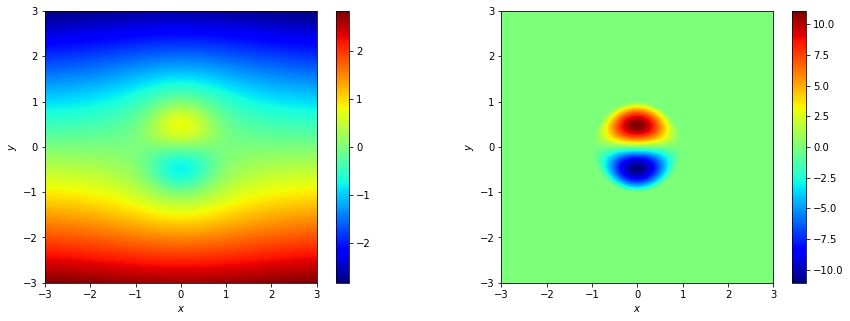
\includegraphics[width=1\textwidth, keepaspectratio]{img/tilt0.png}
    \caption{Initial configuration for the tilt instability showing the dipole current density $\psi_e$ (left panel)
    and the density current $J_e$ (right panel).}
    \label{fig:tilt0}
\end{figure}

Moreover, an initial zero stream function is assumed $\phi_e(x, y) = 0$, with zero initial vorticity
$\omega_e(x, y) = 0$ and we assume $\eta = \nu$ and $\rho = \mu_0 = 1$.
Since we consider an incompressible reduced MHD model, thermal pressure is absent and we are not concerned by such choice.
The initial current structure and current density are reported in Figure \ref{fig:tilt0}.

\subsection{Typical evolution of the tilt instability}

During the early time evolution of the system corresponding to the tilt instability, the pair of
oppositely directed currents tend to repel one another giving rise to a rotation (see Figure \ref{fig:tilt1} 
for a case with $\eta = 3\times 10^{-3}$) during the linear phase. 
The sense of rotation of the structure (anticlockwise in Figure \ref{fig:tilt1}) is not predetermined and depends only on the
numerical noise. This rotation causes two new regions of current density taking the form of two bananas. 

\begin{figure}[h!]
    \centering
    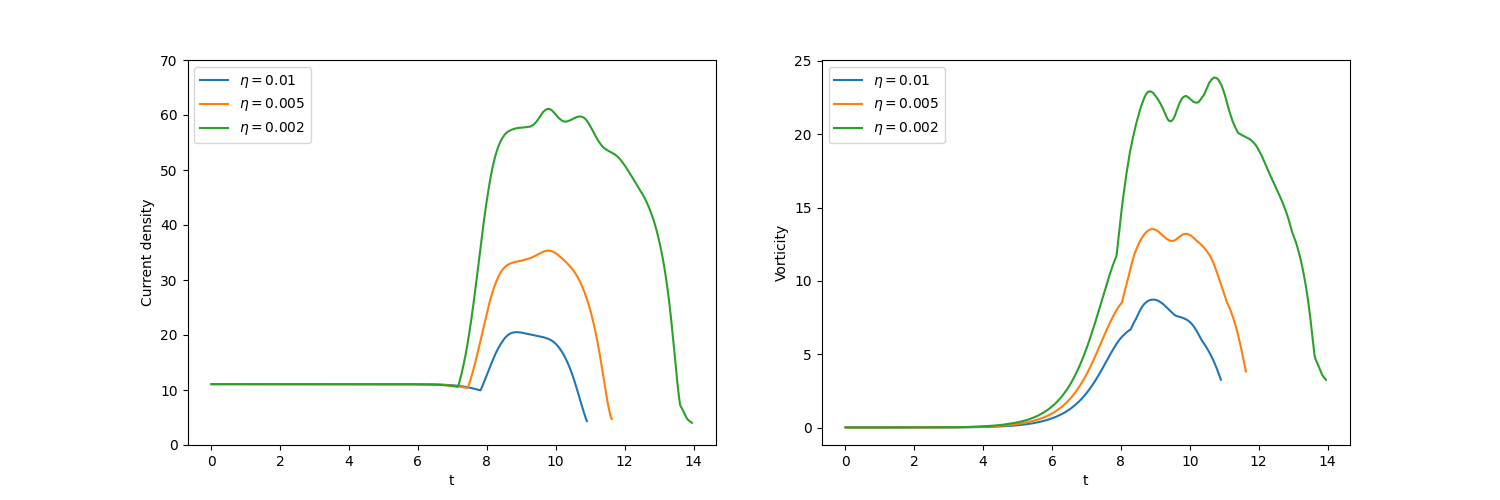
\includegraphics[width=1\textwidth, keepaspectratio]{img/history1.png}
    \caption{Time history of the maximum current density amplitude (left panel) and maximum vorticity amplitude 
    (right panel) for three resistivity values
    $\eta = 0.01, 0.005$ and $0.002$.}
    \label{fig:tilt2}
\end{figure}

\begin{figure}[h!]
    \centering
        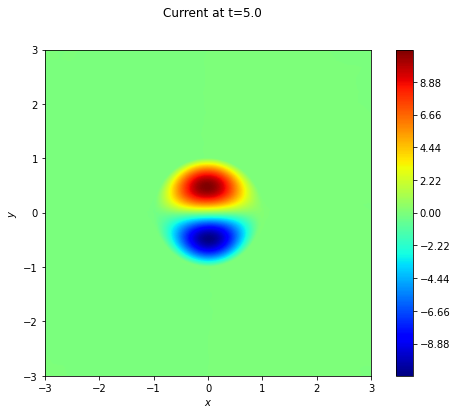
\includegraphics[width=.45\textwidth, height=0.4\textwidth, keepaspectratio]{img/tilt5.png}
        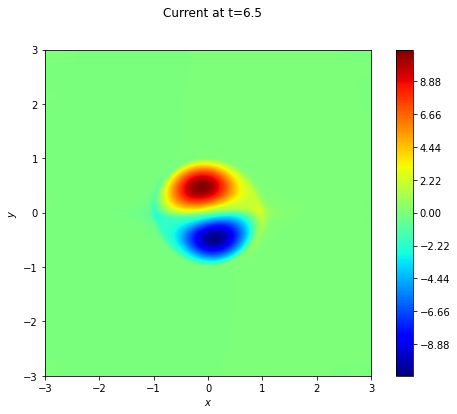
\includegraphics[width=.45\textwidth, height=0.4\textwidth, keepaspectratio]{img/tilt6.png}
        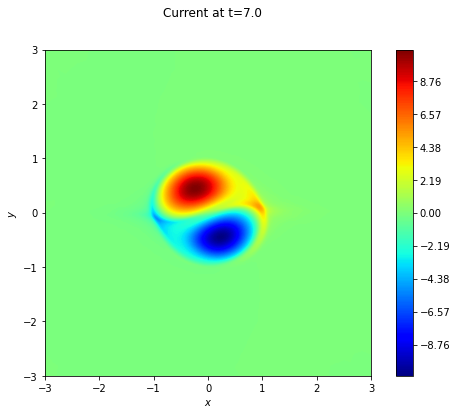
\includegraphics[width=.45\textwidth, height=0.4\textwidth, keepaspectratio]{img/tilt7.png}
        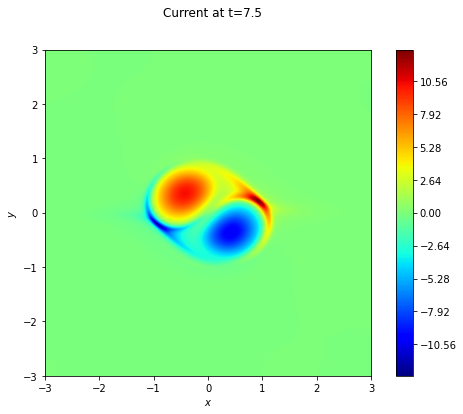
\includegraphics[width=.45\textwidth, height=0.4\textwidth, keepaspectratio]{img/tilt75.png}
        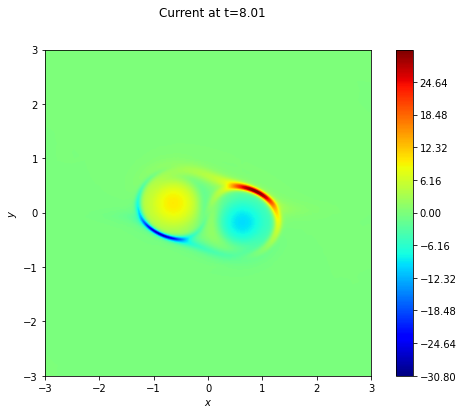
\includegraphics[width=.45\textwidth, height=0.4\textwidth, keepaspectratio]{img/tilt8.png}
        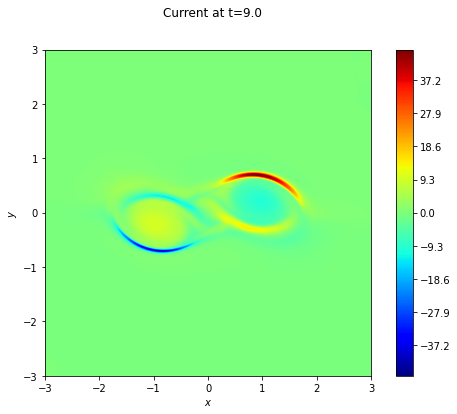
\includegraphics[width=.45\textwidth, height=0.4\textwidth, keepaspectratio]{img/tilt9.png}
        \caption{Current density at different times during the development of the tilt instability for $\eta = 3\times 10^{-3}$.}
    \label{fig:tilt1}
\end{figure}

The time history of the maximum current density amplitude and the maximum vorticity amplitude (taken over the whole domain)
is shown to increase exponentially in time over the equilibrium value, as illustrated in Figure \ref{fig:tilt2} for three different
viscosity values $\eta = 0.01, 0.005$ and $0.002$. A steady-state is obtained with a nearly constant 
current density structure subsequently forming, driving thus the reconnection process.

\clearpage
\section{Numerical results}

In this section, we describe the resolution of the previous tilt problem using PINNs. 
The objective was to reproduce the evolution of the system with PINNs. Using a reference solution given by 
H. Baty (Strasbourg's astronomical observatory), based on finite elements, to check the validity of our solution. 
Unfortunately, it took a lot of time to tune the model's hyperparameters and make the PINNs work so we 
did not have time to design a reduced model that works.
\subsection{Model design}

First of all, we decided to modify the PINNs loss from Equation \ref{eq:LOSS} and remove the 
boundary and initial conditions residual, and add a data misfit term instead. The new loss writes

\begin{align}
    J(\bm \theta) \simeq  \frac{1}{m} \sum_{j=1}^{m} \mathcal{N}[t_j^r,\bbm x_j^r, u_{\bm \theta}(t_j^r,\bbm x_j^r)]^2
    + \underbrace{\frac{\lambda}{N_d} \sum_{j=1}^{N_d} \Big[ u_j^d  - u_{\bm \theta}(t_j^d, \bbm x_j^d) \Big]^2}_{ = J_{\text{data}}(\bm \theta)}
    \label{eq:LOSSMHD}
\end{align}

where $\{t_j^d, \bbm x_j^d \}_{j=1}^{N_d}$ is the set of training data points, $\{u_j^d\}_{j=1}^{N_d}$ represents the values that
the exact solution take on these points and $\lambda$ is a weight parameter used to adjust the relative importance of each term.
The first term on the right hand side of the equation is still the residual of the PDE, while the second one now quantifies
how much the PINNs fits the data. We use this trick because after many attempts, the PINNs was unable to trigger the instability, so 
this is a way to start the simulation at an advanced time in the system evolution. But this trick also helps to guide the training
by imposing the PINNs to take specific value at some points.
In practice, we have several data sets from a high-fidelity simulation at multiple time step.\\

Moreover, we saw in a previous section that the scalar variables involved in the tilt instability, that is $\omega,\phi,J$ and $\psi$,
can take a wide range of values, typically from $10^{-3}$ to $10^2$ for a small viscosity.  In principle, using 
sufficiently wide networks would allow the PINNs to associate different parts of each layer to a specific
output. However, the wide range of values taken by the solution will result in a bad approximate and, after many attempts, 
we find that using separate networks facilitates the training.
Therefore, we used two independent FFNNs blended together as in \cite{HAGHIGHAT2021113741}.
The first one is used to approximate the hydrodynamic variables $\omega$ and $\phi$ while the second
one to approximate the magnetic variables $J$ and $\psi$. Also, we remark that the choice of a specific formulation for 
reduced MHD have no incidence on the training, so we use the flow-vorticity formulation.\\

Finally, assuming that we use $D$ data snapshots, we have to modify the loss in Equation \ref{eq:LOSSMHD}, and add many parameters to 
ponderate the loss between the different scalar variables misfits for each data snapshot. The final data loss $J_{\text{data}}$
writes,

\begin{align}
    J_{\text{data}}(\bm \theta)  
     = \sum_{d=0}^{D} \Big( \frac{\lambda_d^\omega}{N_d} \sum_{j=1}^{N_d} \big[ \omega_j^d  - \hat{\omega}(t_j^d, \bbm x_j^d) \big]^2 
    & + \frac{\lambda_d^\phi}{N_d} \sum_{j=1}^{N_d} \big[ \phi^d  - \hat{\phi}(t_j^d, \bbm x_j^d) \big]^2 \\
    & + \frac{\lambda_d^J}{N_d} \sum_{j=1}^{N_d} \big[ J_j^d  - \hat{J}(t_j^d, \bbm x_j^d) \big]^2 
    + \frac{\lambda_d^\psi}{N_d} \sum_{j=1}^{N_d} \big[ \psi^d  - \hat{\psi}(t_j^d, \bbm x_j^d) \big]^2 \Big)
    \label{eq:LOSSMHD2}
\end{align}
Where terms with a hat are the PINNs prediction, and the lambdas
are weights parameters used to adjust the relative importance of each term, which adds to the $4$ other weights 
corresponding to the four PDEs equations to reach a total of $4\times (D+1)$ hyperparameters to adjust 
for the training process.

\subsection{Results}

We trained two networks with the same architecture :  16-layers FFNN with 256 neurons
in each hidden layer. The first one corresponding to the hydrodynamic variables use the ReLu activation function 
while the other, corresponding to the magnetic variables use the hyperbolic tangent function. 
We trained the PINNS with the following hyperparameters : batch size is set to 3,000, the learning rates 
for the two optimizers are the same, and were initially set to $10^{-3}$ and follows an exponential decay of factor $0.98$ every $200$ step.
Also we set the resistivity $\eta = 3\times 10^{-3}$, used $10,000,000$ collocation points and $10$ different data snapshots 
regularly spaced in time , corresponding to  
the beginning of the exponential croissance phase ($t = 4$) until the reconnection process ($t=10$).\\

The tuning of all the hyperparameters, in particular the weights parameters between the different terms in the loss, 
was a long and tedious task. 
Indeed, the PDE system we look is highly non-linear, the functions we want to approximate take complex shapes that evolve a lot, and 
take wide range of values. But we finally manage to obtain good approximations.\\

Figure \ref{fig:tilt3} compares PINNs prediction to the real solution data. 
It shows the time history of the maximum current density amplitude and maximum vorticity amplitude on the 
left hand side, and the value of kinetic and magnetic energy of the system on the right hand side, computed using the formula 

\begin{equation}
    E_{\text{cin}}(t) = \frac{1}{2} \int_\Omega |\nabla \phi(t,\bbm x) | ^2 \mathrm{d}\bbm x \quad  
    \text{and} \quad E_{\text{mag}}(t) = \frac{1}{2} \int_\Omega |\nabla \psi (t,\bbm x)| ^2 \mathrm{d}\bbm x
\end{equation}
We can see that the PINNs prediction is able to predict the evolution of the system with a relatively good accuracy on $J$ and $\omega$, 
but for the two others, $\phi$ and $\psi$, involved in the kinetic and magnetic energy, the approximate seems to have a lower accuracy.\\

Figures \ref{fig:tilt4}, \ref{fig:tilt5}, \ref{fig:tilt6} and \ref{fig:tilt7} show 
the PINNs prediction for the different scalar fields compared to the real solutions at 
different time step, $t=5, 6, 7.5$ and $9$. These figures confirm that the PINNs have no difficulty to approximate the 
main variables ($\omega$ and $J$) but face greater difficulties to catch the dynamic of the other variables ($\phi$ and $\psi$).\\

\begin{figure}[h!]
    \centering
    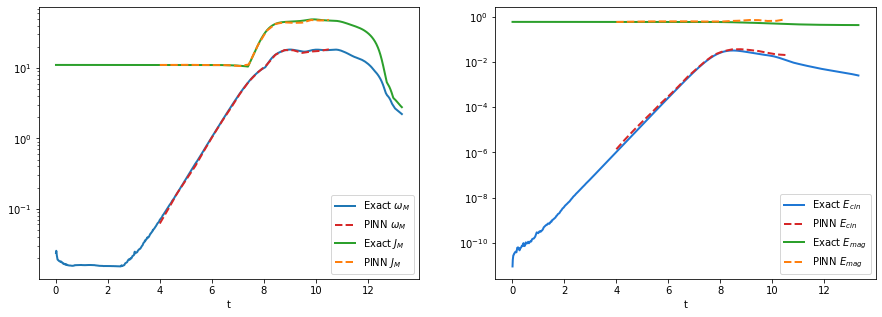
\includegraphics[width=.9\textwidth, keepaspectratio]{img/courbeMHD.png}
    \caption{Comparison of the time history of the maximum current density amplitude and maximum vorticity amplitude (left panel)
    and the kinetic and magnetic energy
    (right panel) between the PINNs prediction and the data.}
    \label{fig:tilt3}
\end{figure}


To conclude, PINNs can solve complex problems, like the tilt problem, without any mesh generation. This is a big advantage
of PINNs over classical numerical methods. Indeed, in \cite{Baty_2019}, author had to implement a highly adaptive characteristic-Galerkin 
scheme that use a finite element discretization 
using triangles with quadratic basis functions on an unstructured grid.

However, we see that PINNs struggle with multi-scale problem like the tilt problem. In these situation, tuning the many training 
hyperparameters is essential otherwise the PINNs will not be able to traing properly, but this a hard task, especially when training
can take hours.

\begin{figure}[h!]
    \centering
        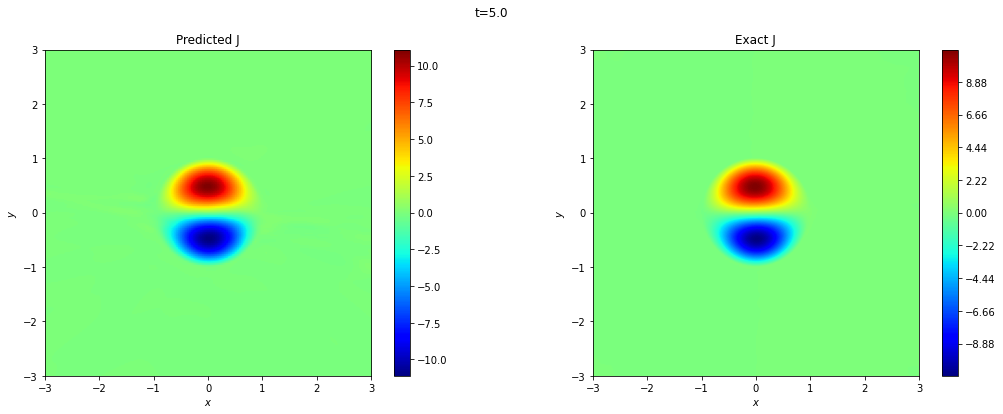
\includegraphics[width=.8\textwidth, height=0.4\textwidth, keepaspectratio]{img/tiltfinal_5.png}
        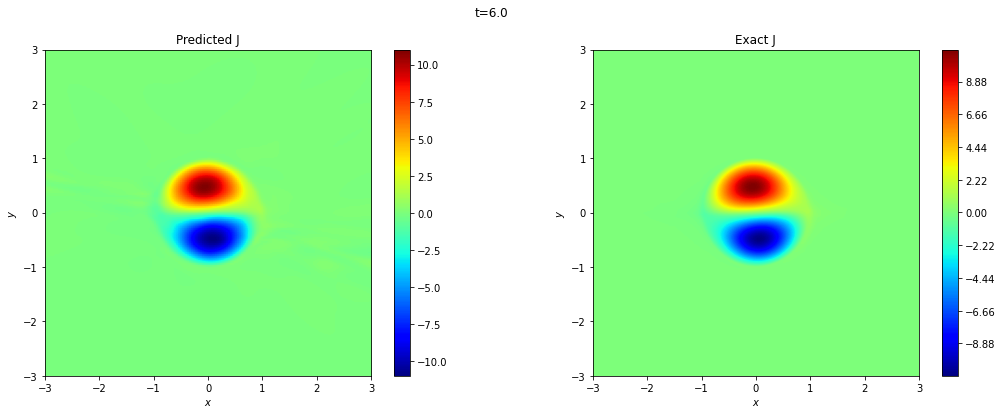
\includegraphics[width=.8\textwidth, height=0.4\textwidth, keepaspectratio]{img/tiltfinal_6.png}
        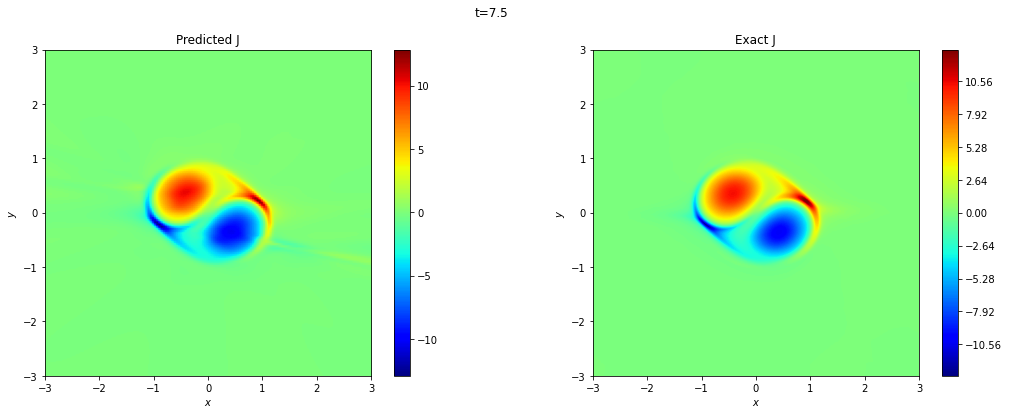
\includegraphics[width=.8\textwidth, height=0.4\textwidth, keepaspectratio]{img/tiltfinal_7.5.png}
        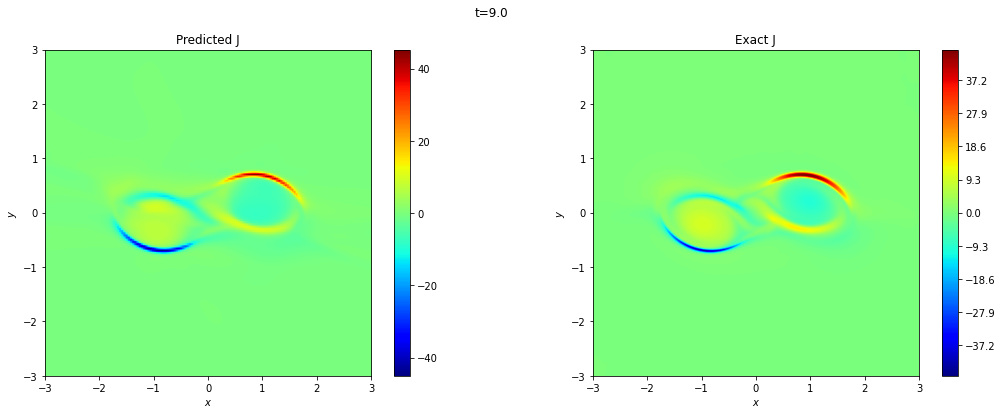
\includegraphics[width=.8\textwidth, height=0.4\textwidth, keepaspectratio]{img/tiltfinal_9.png}
        \caption{Current density predicted by PINNs compared to the exact solution at different times. $\eta = 3\times 10^{-3}$.}
    \label{fig:tilt4}
\end{figure}

\begin{figure}[h!]
    \centering
        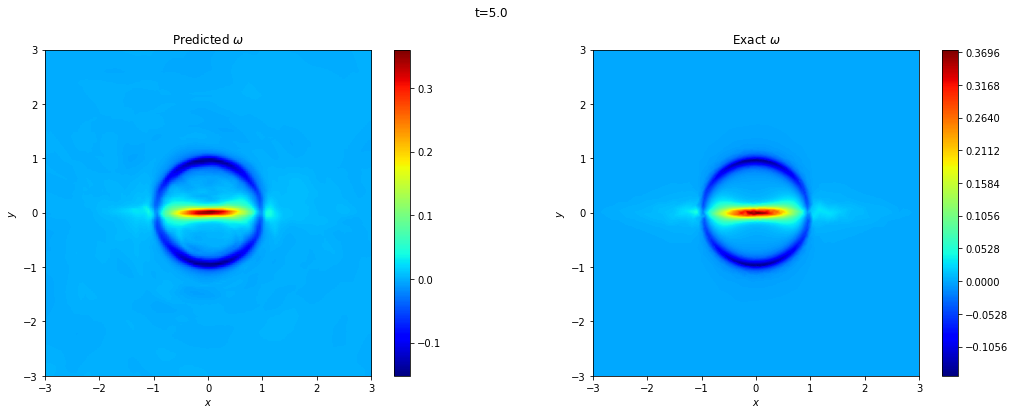
\includegraphics[width=.8\textwidth, height=0.4\textwidth, keepaspectratio]{img/tiltfinalO_5.png}
        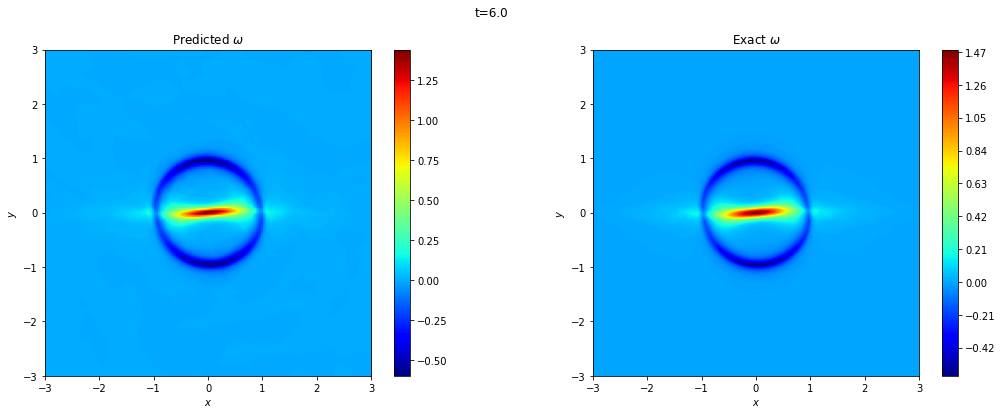
\includegraphics[width=.8\textwidth, height=0.4\textwidth, keepaspectratio]{img/tiltfinalO_6.png}
        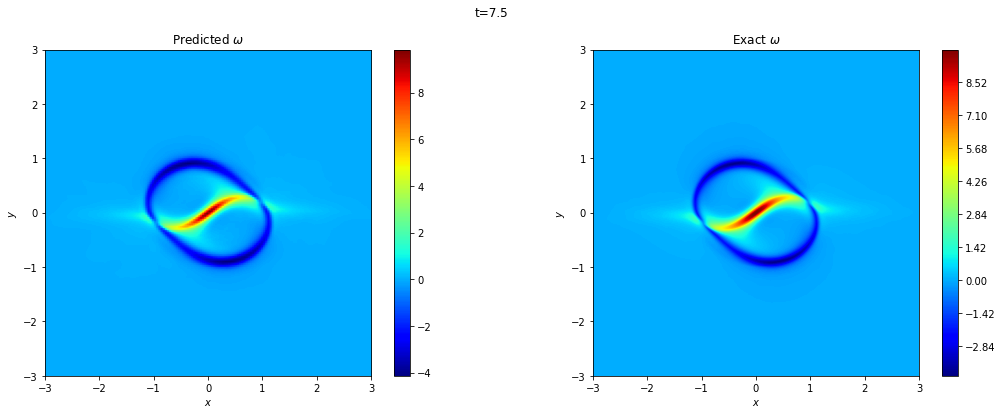
\includegraphics[width=.8\textwidth, height=0.4\textwidth, keepaspectratio]{img/tiltfinalO_7.5.png}
        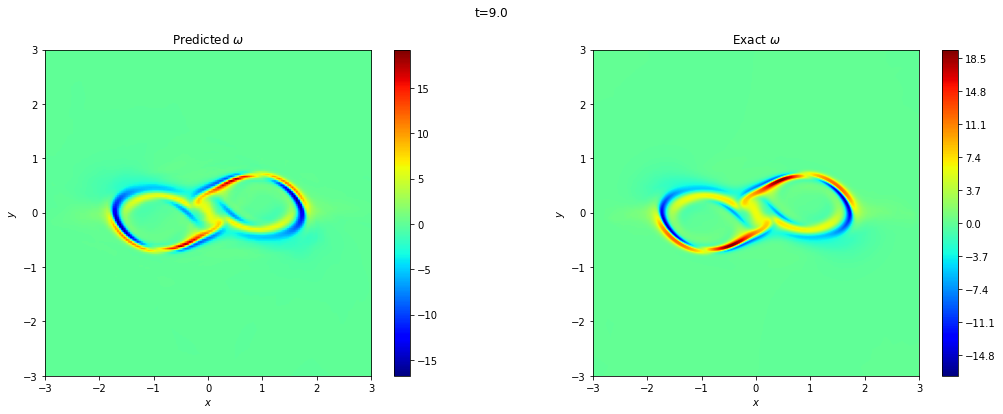
\includegraphics[width=.8\textwidth, height=0.4\textwidth, keepaspectratio]{img/tiltfinalO_9.png}
        \caption{vorticity predicted by PINNs compared to the exact solution at different times. $\eta = 3\times 10^{-3}$.}
    \label{fig:tilt5}
\end{figure}

\begin{figure}[h!]
    \centering
        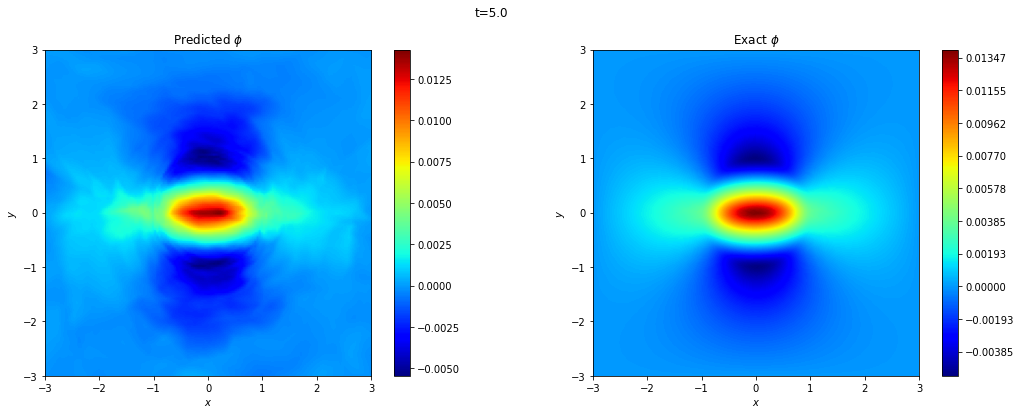
\includegraphics[width=.8\textwidth, height=0.4\textwidth, keepaspectratio]{img/tiltfinalPHI_5.png}
        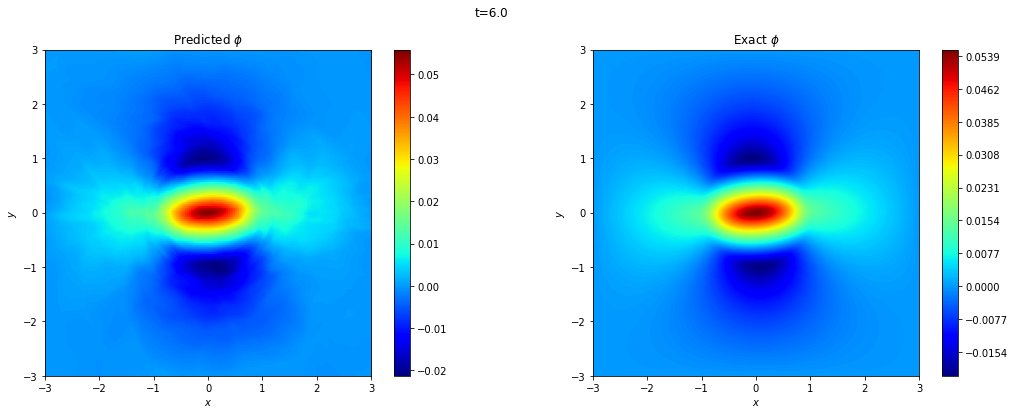
\includegraphics[width=.8\textwidth, height=0.4\textwidth, keepaspectratio]{img/tiltfinalPHI_6.png}
        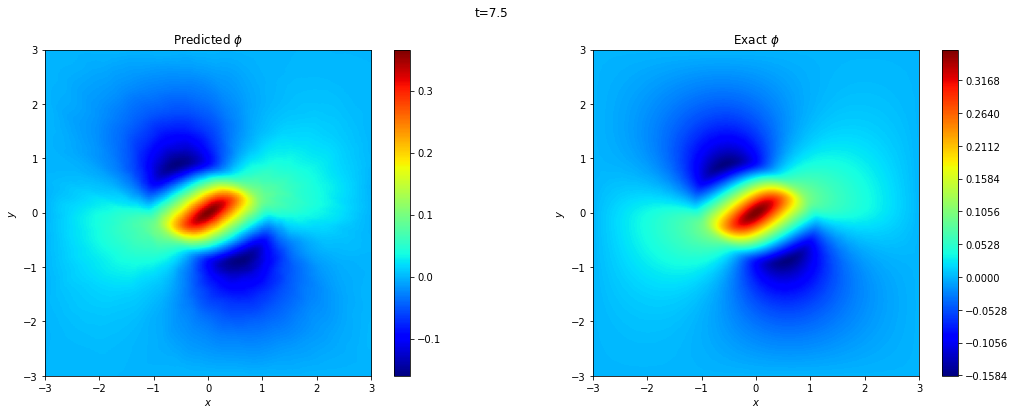
\includegraphics[width=.8\textwidth, height=0.4\textwidth, keepaspectratio]{img/tiltfinalPHI_7.5.png}
        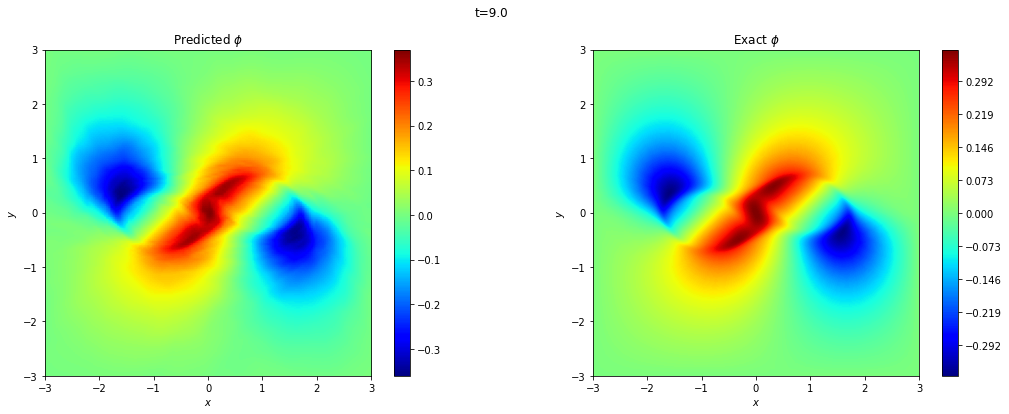
\includegraphics[width=.8\textwidth, height=0.4\textwidth, keepaspectratio]{img/tiltfinalPHI_9.png}
        \caption{$\phi$ function predicted by PINNs compared to the exact solution at different times. $\eta = 3\times 10^{-3}$.}
    \label{fig:tilt6}
\end{figure}

\begin{figure}[h!]
    \centering
        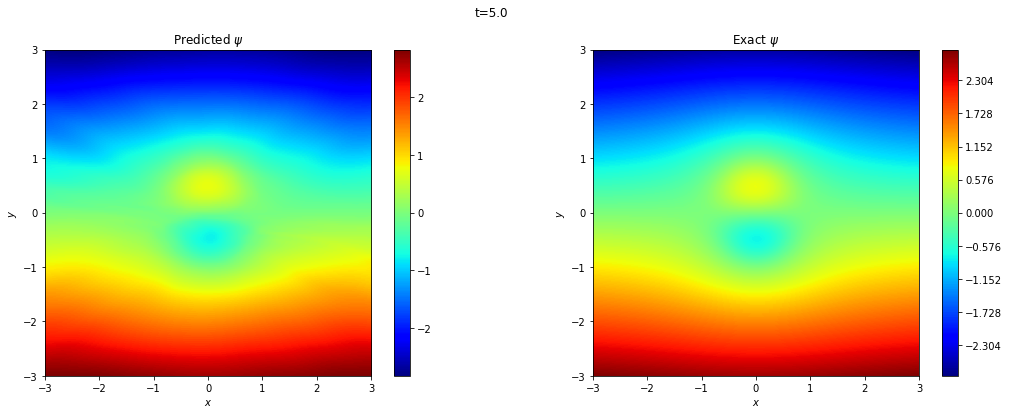
\includegraphics[width=.8\textwidth, height=0.4\textwidth, keepaspectratio]{img/tiltfinalPSI_5.png}
        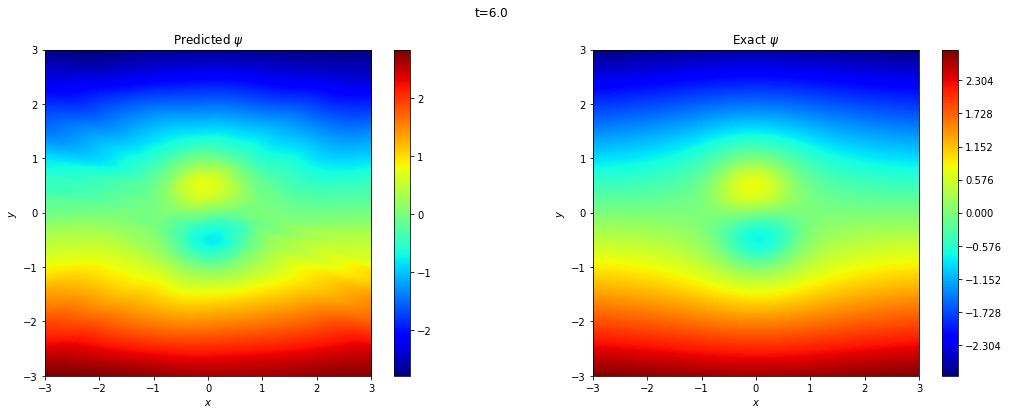
\includegraphics[width=.8\textwidth, height=0.4\textwidth, keepaspectratio]{img/tiltfinalPSI_6.png}
        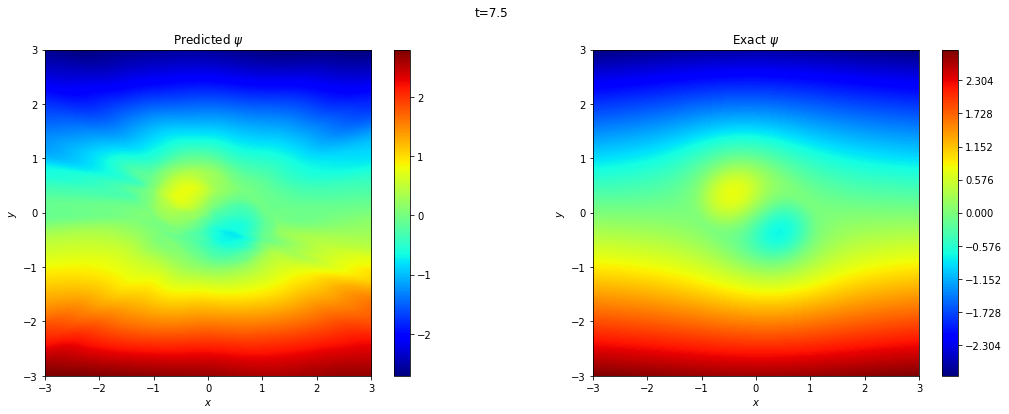
\includegraphics[width=.8\textwidth, height=0.4\textwidth, keepaspectratio]{img/tiltfinalPSI_7.5.png}
        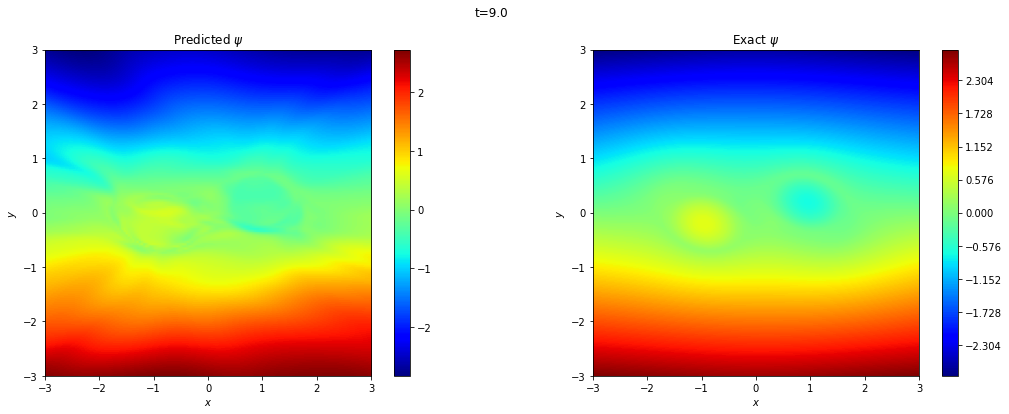
\includegraphics[width=.8\textwidth, height=0.4\textwidth, keepaspectratio]{img/tiltfinalPSI_9.png}
        \caption{$\psi$ function predicted by PINNs compared to the exact solution at different times. $\eta = 3\times 10^{-3}$.}
    \label{fig:tilt7}
\end{figure}

%%%%%%%%%%%%%%%%%%%%%%%%%%%%%%%%%%%%%%%%%%%%%%%%%%%%%%%%%%%%%%%%%%%%%%
\clearpage

%%%%%%%%%%%%%%%%%%%%%%%%%%%%%%%%%%%%%%%%%%%%%%%%%%%%%%%%%%%%%%%%%%%%%%
%%%%%%%%%%%%%%%%%%%%%%%%%%%%%%%%%%%%%%%%%%%%%%%%%%%%%%%%%%%%%%%%%%%%%%
\backmatter

\clearpage
\nocite{*}
\bibliographystyle{apalike}
\bibliography{report}

\end{document}